% Placeholder preamble: replace \documentclass and packages with the venue style.
\documentclass[11pt]{article}

% Change "review" to "final" to generate the final (sometimes called camera-ready) version.
% Change to "preprint" to generate a non-anonymous version with page numbers.
\usepackage[review]{acl}

% Standard package includes
\usepackage{times}
\usepackage{latexsym}

% For proper rendering and hyphenation of words containing Latin characters (including in bib files)
\usepackage[T1]{fontenc}
% For Vietnamese characters
% \usepackage[T5]{fontenc}
% See https://www.latex-project.org/help/documentation/encguide.pdf for other character sets

% This assumes your files are encoded as UTF8
\usepackage[utf8]{inputenc}

% This is not strictly necessary, and may be commented out,
% but it will improve the layout of the manuscript,
% and will typically save some space.
\usepackage{microtype}

% This is also not strictly necessary.
% However, it will improve the aesthetics of text in
% the typewriter font.
\usepackage{inconsolata}

%Including images in your LaTeX document requires adding
%additional package(s)
\usepackage{amsmath,amssymb}
\usepackage{booktabs}
\usepackage{graphicx}
\usepackage{multirow}
\usepackage{xcolor}
\usepackage{natbib}
\usepackage{hyperref}
\usepackage[capitalize]{cleveref}
\graphicspath{{figures/}}

\newcommand{\musique}{MuSiQue}
\newcommand{\twowiki}{2WikiMultiHopQA}
\newcommand{\vdm}{v_{\mathrm{dm}}}
\newcommand{\vlr}{v_{\mathrm{lr}}}

\title{The Evidence Within: Evidence Sufficiency and Uptake in the Residual Stream of Retrieval-Augmented LLMs}
\author{Iacopo Ghinassi, Mingye Zhu}
\date{}

\begin{document}
\maketitle

\begin{abstract}
Retrieval-augmented language models receive evidence piece by piece, and at some point that evidence becomes enough to answer the question. We ask whether the model's internal state registers this moment, and whether it also registers whether the model will actually use the evidence. We build evidence trajectories for multi-hop questions: each gold paragraph is added in turn, and every decisive addition is paired with matched additions of irrelevant, duplicate or falsified paragraphs to the same starting context. Linear probes on the residual stream at the answer position, read before any token is generated, recognise the decisive addition at $0.95$ AUROC in three model families and predict whether the model will take up the decisive evidence rather than ignore it at $0.78$. We compare these readouts with the baselines a practitioner would otherwise use. For sufficiency, the internal state is far more reliable than the model's own verbalised judgement ($0.98$ against $0.71$--$0.77$ AUROC with paragraph count matched): the models declare complete evidence insufficient a third of the time, and the probe recovers most of those cases. For uptake, text classifiers stay near chance, whether the model answers at all already predicts much of it, and the internal state adds to that signal and is the best single predictor of correctness among the answers the model gives. The probe directions turn out to be readouts rather than levers: steering along them changes nothing, whereas the difference between the mean sufficient and insufficient states acts as a gate on abstention. The readouts replicate on HotpotQA, on RAGBench's naturally retrieved documents across five domains, on a synthetic benchmark and on BM25- and E5-retrieved Wikipedia evidence, with directions learned on Wikipedia transferring only partially to other domains.
\end{abstract}

\section{Introduction}
\label{sec:intro}
Retrieval-Augmented Generation (RAG) grounds the answers of a Large Language Model (LLM) in retrieved evidence \cite{NEURIPS2020_6b493230}. In practice the evidence rarely arrives all at once. A retriever returns passages of mixed relevance, an agent fetches them over several rounds, and for multi-hop questions the answer depends on several separate facts that may be retrieved at different times \cite{trivedi2022musique}. Two questions then matter at every step. Is the evidence now \emph{sufficient} to answer? And, if it is, will the model actually \emph{take it up}, or will it ignore the decisive passage and answer as before? Today both questions are usually put to the model itself: it is told to say ``INSUFFICIENT'' when it cannot answer, and its output is taken as the verdict.

This paper asks whether the model's internal state gives a better answer. Prior work has shown that residual-stream activations carry information about the conflict between retrieved context and parametric memory, and about how much the model relies on the context \cite{SpARE,context-vs-memory}. Nothing comparable exists for sufficiency and uptake, and we know of no study that compares an internal readout of these properties with the model's own verbalised judgement, or with a text classifier given the same input.

We study this with \emph{evidence trajectories}. For every multi-hop question we add the gold paragraphs one at a time and run a fresh forward pass on each context, reading the residual stream at the position that produces the first answer token, before anything is generated. The addition that makes the evidence complete, the \emph{decisive increment}, is paired with controls that add, to the same starting context, a distractor of the same length, a duplicate of a paragraph already present, a falsified version of the missing paragraph, or an irrelevant paragraph that mentions the answer string. A probe trained to tell the decisive increment from these controls cannot rely on length, on the presence of the answer string or on lexical relevance alone. Every increment is also labelled with what the model's answer did, so a second probe, trained on decisive increments only, predicts uptake: whether the answer becomes correct, or the new evidence is ignored.

Our findings are, in order of importance, the following. First, sufficiency and uptake are both linearly readable before generation, at $0.95$ and $0.78$ AUROC, on splits that keep supporting documents, answer entities and relation types disjoint between training and test. Second, these readouts compare favourably with the alternatives. For sufficiency the internal state is far more accurate than the model's verbalised judgement, which declares complete evidence insufficient a third of the time, and somewhat more accurate than a text classifier that sees the whole context. For uptake no text classifier gets far above chance; the model's decision to answer at all predicts it about as well as the probe does, and the probe adds to that decision and is the best single predictor of whether an answer the model gives is correct. Third, as a corollary, the probe directions are not levers: steering, patching and projecting along them leave behaviour unchanged. The one direction with a causal effect is the difference between the mean sufficient and insufficient states, and it acts as a gate on abstention rather than on evidence use, which connects our results to work on steering abstention through confidence directions \cite{ActivationSteering,Kumaran2026}. Fourth, the readouts are recoverable in three model families and on other datasets, and directions learned on \musique{} transfer to HotpotQA almost intact but only partially to RAGBench's naturally retrieved documents and to synthetic evidence.

Our contributions are as follows.
\begin{itemize}
  \item \textbf{An increment-based protocol} for reading evidence sufficiency and evidence uptake from a single forward pass before generation, with matched controls that rule out the surface explanations.
  \item \textbf{A comparison with the baselines that matter}: text classifiers on the same inputs, and the model's own verbalised judgement and confidence. It shows where the internal state adds information and where it does not. As a corollary, we show that the probe directions are readouts rather than mechanisms, and that the mean-difference direction is a steerable abstention gate.
  \item \textbf{Generalisation} to Llama and Mistral, to HotpotQA \cite{yang2018hotpotqa}, to RAGBench \cite{friel2024ragbench} across five domains, to a synthetic benchmark with paraphrased, partial and contradictory evidence, and to retrieved rather than curated evidence. We release the Evidence State Transition Benchmark (ESTB), which collects these sources under one labelling scheme, together with our code.
\end{itemize}

\section{Related work}
\label{sec:related}
% To be written by the authors.

\section{Experimental setup}
\label{sec:setup}

\paragraph{Data.}
We need questions whose answer depends on several separate facts, with annotations saying which paragraphs contain them. A context is then \emph{sufficient} exactly when it contains every gold paragraph, so sufficiency is defined by the construction and not by the model's behaviour. Multi-hop question answering provides this. Our main experiments use the 2-hop questions of \musique{} \cite{trivedi2022musique}, which composes single-hop questions so that every hop is needed, and gives one gold Wikipedia paragraph per hop, the sub-question and sub-answer of each hop, and 18 distractor paragraphs. For each model we screen 4{,}000 questions without any evidence and keep 2{,}000 that the model answers incorrectly, so that a correct answer after evidence is added can be attributed to the evidence. \Cref{sec:external} adds \twowiki{} \cite{ho2020constructing}, 3--4-hop \musique{}, HotpotQA \cite{yang2018hotpotqa}, RAGBench \cite{friel2024ragbench}, whose documents were retrieved by real RAG pipelines in five domains, and a synthetic benchmark over fictional entities.

\paragraph{Models.}
Qwen2.5-7B-Instruct (28 layers, $d=3584$), Llama-3.1-8B-Instruct (32 layers, $d=4096$) and Mistral-7B-Instruct-v0.3 (32 layers, $d=4096$), in bfloat16, with greedy decoding of at most 16 tokens and each model's chat template.

\paragraph{Prompt and anchor.}
Every context is shown with the same instruction: ``Use only the supplied evidence to answer the question. If the evidence is insufficient, output INSUFFICIENT.'' The model therefore makes an explicit sufficiency judgement in its output, which we later use as a baseline. We read the residual stream after every decoder block at the last prompt token, the position from which the first answer token is predicted, so all readouts are taken before generation. A second instruction that lets the model use its own knowledge as well gives the same results (\cref{app:augmented}).

\paragraph{Evidence trajectories.}
For each question we build a family of contexts; \cref{app:conditions} lists them all. Writing $g_1,\dots,g_n$ for the gold paragraphs, we start from the empty context and from a context of $n$ distractors matched in length to the gold paragraphs. We then add the gold paragraphs one at a time, in the hop order of the dataset and in reverse order. The context that receives the last gold paragraph is the \emph{minimal sufficient} context. Every context that lacks exactly one gold paragraph, which we call \emph{penultimate}, also receives four alternative additions: a distractor of the same length as the missing paragraph, a duplicate of a gold paragraph already present, a falsified copy of the missing paragraph in which the hop's sub-answer is replaced by another question's sub-answer of the same type, and a distractor to which the sentence ``not to be confused with \{answer\}'' is appended. Finally, the minimal sufficient context receives a further distractor, a duplicate gold paragraph, a conflicting falsified paragraph, and the full set of 20 paragraphs. New paragraphs are inserted at a random position, so the position of the decisive paragraph carries no information. For a 2-hop question this gives 17 contexts.

\paragraph{Increments and tasks.}
An \emph{increment} is a pair of contexts $C_{k-1}\subset C_k$ that differ by one addition. The \emph{decisive} increment adds the last missing gold paragraph. The other increments add a gold paragraph that still leaves one missing (\emph{non-decisive}), or something \emph{irrelevant} to sufficiency: a distractor, a duplicate, a falsified paragraph, an answer-string control, or any addition to a context that is already sufficient. \Cref{tab:tasks} summarises how the two tasks use them; the full list of increment kinds is in \cref{app:conditions}. \emph{Sufficiency} asks whether an increment is the decisive one. Its positives are the decisive increments and its negatives all the others; the \emph{matched} version keeps only the four controls built from the same penultimate context, which is the harder comparison. \emph{Uptake} is defined on decisive increments only, by what the model's answer does: it is positive when the answer becomes correct and negative when the model still answers wrongly or says INSUFFICIENT. Correctness is exact match on any alias, or containment within a short prediction. Every increment also carries the model's full behavioural transition, which defines three further tasks, correction, stability and revision, reported in \cref{app:related}.

\begin{table}[t]
\centering\footnotesize
\setlength{\tabcolsep}{3pt}
\begin{tabular}{@{}lp{1.7cm}p{3.55cm}@{}}
\toprule
Task & Positive increments & Negative increments \\
\midrule
Sufficiency & decisive & non-decisive gold paragraph; irrelevant additions (distractor, duplicate, falsified, answer string); additions after sufficiency \\
\;\;matched & decisive & the four irrelevant additions made to the same penultimate context \\
Uptake & decisive, answer becomes correct & decisive, answer stays wrong or INSUFFICIENT \\
\bottomrule
\end{tabular}
\caption{The two tasks and the increments that define them. \Cref{tab:kinds} in \cref{app:conditions} gives the complete list.}
\label{tab:tasks}
\end{table}

\paragraph{Behaviour.}
The models follow the instruction when the evidence is clearly lacking: they say INSUFFICIENT on 94--97\% of distractor-only contexts. On the minimal sufficient context they answer correctly only 36--47\% of the time and say INSUFFICIENT 30--36\% of the time, so the verbalised judgement is often wrong on complete evidence; a falsified final paragraph halves abstention (\cref{tab:behaviour}, \cref{app:behaviour}).

\paragraph{Splits.}
Probes are trained on 70\% of the questions and tested on the rest. By default we use the \emph{document split}, in which questions that share a supporting Wikipedia page are kept on the same side, so a probe cannot succeed by memorising facts about specific pages. Splits by question, by answer entity and by relation type give the same results (\cref{app:splits}).

\paragraph{Baselines.}
Two kinds of baseline are run on exactly the same increments, labels and splits. \emph{Text classifiers} see the input but not the model: a TF-IDF logistic regression and a fine-tuned DeBERTa-v3-base cross-encoder \cite{he2023debertav3}, each given the question and the added paragraph, the latter also with the previous context (\cref{app:probing}). \emph{Self-verbalisation} uses the model's own output: whether it answers rather than saying INSUFFICIENT, and its confidence, measured as the top-token probability or the negative entropy at the anchor.

\section{Method}
\label{sec:method}

\paragraph{Paired updates and probes.}
Let $h^{(l)}(C)\in\mathbb R^{d}$ be the residual stream after block $l$ at the anchor for context $C$. For the increment $C_{k-1}\to C_k$ we form the paired update $\Delta h^{(l)}=h^{(l)}(C_k)-h^{(l)}(C_{k-1})$, which isolates what the added paragraph did to the model's state and removes the content that both contexts share. For each task and layer we fit an $\ell_2$-regularised logistic regression on standardised updates with class balancing. We probe every layer and report the one selected by grouped three-fold cross-validation on the training questions only; the depth profile is in \cref{app:readout}. The probe direction is the weight vector mapped back to activation space and normalised. We also compute the \emph{difference-of-means} direction $\vdm\propto\mathbb E[\Delta h\mid y{=}1]-\mathbb E[\Delta h\mid y{=}0]$ and, for comparison, probes on the raw states $h(C_{k-1})$ and $h(C_k)$ (\cref{app:rep}).

\paragraph{Nuisance analysis.}
A paired update also reflects surface properties of the increment: how much text was added, whether it mentions the answer, how lexically relevant it is to the question, where it was inserted, and how much the model's output distribution moved. We collect these into a \emph{nuisance vector} $z$ per increment (the full list is in \cref{app:probing}) and run two tests. A classifier that sees only $z$ measures how far surface properties alone go. The \emph{gain} is the AUROC added when the probe score, computed out of fold on training increments, is given to that classifier as an extra feature; it measures what the activations contribute beyond those properties.

\paragraph{Generalisation.}
Directions are learned on the training questions of 2-hop \musique{} and then applied, without retraining and at the layer chosen there, to other settings: a conversational protocol in which the model sees its previous answer before the new paragraph, \twowiki{}, 3--4-hop \musique{}, and the external benchmarks of \cref{sec:external}. Where the target has its own trajectories we also train probes on it, which gives the ceiling for transfer. Hidden sizes differ across model families, so there we replicate the whole procedure instead of transferring vectors.

\paragraph{Causal tests.}
A direction from which a property can be read is not necessarily one the model uses. We therefore ask three questions of a direction $v$, on 150 held-out questions, each with an \emph{insufficient} prompt that lacks one gold paragraph and the \emph{sufficient} prompt in which it has been added. \emph{Does pushing along $v$ change behaviour?} Steering adds $\alpha\,u\,v$ to the residual at the anchor and at every generated position, where $u$ is the gap between the sufficient and insufficient means along $v$, so that $\alpha=1$ moves the activation by one such gap; a random direction of the same norm is the control. \emph{Does the model need $v$?} Projection-out takes the sufficient prompt and sets its component along $v$ to the insufficient-state mean, from the chosen layer onward; if the model relied on $v$, it should start abstaining. \emph{Where in the update does the causal content lie?} Patching runs the insufficient prompt with its anchor residual replaced by the sufficient prompt's, either in full, or only in the component along $v$, or only in the component orthogonal to $v$; further variants restrict the replacement to a random subspace, to the top principal components of training updates, or to the unembedding direction of the gold answer's first token (\cref{app:probing}). Outcomes are the rate at which the model answers rather than saying INSUFFICIENT and the rate of correct answers. We test the logistic probe direction $\vlr$ and the difference-of-means direction $\vdm$ \cite{marks2023geometry,ActivationSteering,meng2022locating}.

\section{Reading sufficiency and uptake before generation}
\label{sec:readout}

Every number in this section is the AUROC of a probe on held-out questions of the document split, at the layer chosen by cross-validation on the training questions.

\begin{table*}[t]
\centering\small
\setlength{\tabcolsep}{3pt}
\begin{tabular}{lccccccccc}
\toprule
& \multicolumn{3}{c}{Qwen2.5-7B} & \multicolumn{3}{c}{Llama-3.1-8B} & \multicolumn{3}{c}{Mistral-7B} \\
\cmidrule(lr){2-4}\cmidrule(lr){5-7}\cmidrule(lr){8-10}
Task & AUROC [95\% CI] & nuis. & gain & AUROC [95\% CI] & nuis. & gain & AUROC [95\% CI] & nuis. & gain \\
\midrule
Sufficiency & 0.948 [0.94,0.95] & 0.87 & 0.11 & 0.952 [0.95,0.96] & 0.86 & 0.12 & 0.949 [0.94,0.95] & 0.87 & 0.11 \\
Sufficiency (matched) & 0.911 [0.90,0.92] & 0.90 & 0.07 & 0.918 [0.91,0.93] & 0.89 & 0.08 & 0.910 [0.90,0.92] & 0.90 & 0.07 \\
Uptake & 0.775 [0.74,0.80] & 0.66 & 0.14 & 0.783 [0.75,0.81] & 0.58 & 0.21 & 0.771 [0.74,0.80] & 0.59 & 0.18 \\
\bottomrule
\end{tabular}

\caption{Held-out AUROC of the probe on paired updates $\Delta h$ (document split; 95\% question-level bootstrap intervals). ``nuis.'': a classifier that sees only surface properties of the increment (length change, presence of the answer string, lexical relevance, change in output confidence). ``gain'': AUROC added when the probe score is given to that classifier.}
\label{tab:probes}
\end{table*}

\paragraph{Sufficiency.}
A probe trained to recognise the decisive increment separates it from all other increments at $0.948$--$0.952$ AUROC in the three models (\cref{tab:probes}). Against the matched controls alone, which start from the same penultimate context and add a distractor, a duplicate, a falsified paragraph or an answer-string control instead of the missing paragraph, it still reaches $0.91$--$0.92$. Surface properties do not explain this. A classifier on the nuisance vector reaches $0.86$--$0.87$, the probe adds $0.11$--$0.12$ on top of it, and a probe trained after the nuisance covariates have been regressed out of the activations still reaches $0.94$--$0.96$. The result is the same under question-, answer- and relation-disjoint splits ($0.94$--$0.96$, \cref{app:splits}). The signal is strongest at 50--60\% of the network's depth, and projections onto the direction order the increment kinds as one would expect if it encoded ``the evidence has just become complete'': decisive first, then falsified, distractor, duplicate and answer-string additions, with additions to an already sufficient context far below (\cref{app:readout}).

\paragraph{Uptake.}
Among decisive increments, a second probe predicts whether the model will use the new paragraph, that is, whether its answer becomes correct, at $0.77$--$0.78$ ($0.85$--$0.87$ on the question split), at layers near the end of the network. This is the task on which the activations add most beyond surface properties: the nuisance classifier reaches only $0.58$--$0.66$ and the probe adds $0.14$--$0.21$. Uptake is a different signal from sufficiency. The two directions are nearly orthogonal (cosine $0.02$--$0.03$), and the sufficiency direction, used to predict uptake, scores only $0.54$--$0.60$.

\paragraph{State or update?}
One may ask whether the subtraction in $\Delta h$ matters. Refitting the probes on the raw state after the addition, $h(C_k)$, gives $0.93$--$0.94$ for sufficiency and $0.77$--$0.80$ for uptake, and a probe on the concatenation of both states matches $\Delta h$; the state before the addition is uninformative beyond the stage of the trajectory it belongs to (\cref{app:rep}). The information therefore sits in the model's state after it has seen the evidence. The paired update is a controlled way of reading it: it discards what both contexts share and lets every decisive increment be compared with controls from the same starting point.

\subsection{Do internal states beat the obvious baselines?}
\label{sec:text}
A practitioner who wants to know whether the evidence is sufficient, or whether the model will use it, has two cheaper options: a text classifier on the same input, or the model's own output, which under our instruction is an explicit verdict on sufficiency. \Cref{tab:baselines} compares both with the probe on the same test increments.

\begin{table*}[t]
\centering\small
\setlength{\tabcolsep}{2.5pt}
\begin{tabular}{llcccccc}
\toprule
& & \multicolumn{3}{c}{text classifiers} & \multicolumn{2}{c}{the model's own output} & \\
\cmidrule(lr){3-5}\cmidrule(lr){6-7}
Model & Task & TF-IDF & DeBERTa (q+added) & DeBERTa (+context) & verbalised & confidence & probe \\
\midrule
Qwen2.5-7B & sufficiency & 0.623 & 0.723 & 0.900 & 0.685 & 0.428 & 0.948 \\
 & sufficiency (matched) & 0.623 & 0.758 & 0.823 & 0.721 & 0.408 & 0.911 \\
 & uptake & 0.574 & 0.569 & 0.557 & 0.776 & 0.571 & 0.775 \\
\midrule
Llama-3.1-8B & sufficiency & 0.625 & 0.715 & 0.888 & 0.692 & 0.409 & 0.952 \\
 & sufficiency (matched) & -- & -- & -- & 0.726 & 0.390 & 0.918 \\
 & uptake & 0.463 & 0.466 & 0.517 & 0.783 & 0.566 & 0.783 \\
\midrule
Mistral-7B & sufficiency & 0.625 & 0.730 & 0.920 & 0.646 & 0.452 & 0.949 \\
 & sufficiency (matched) & -- & -- & -- & 0.671 & 0.428 & 0.910 \\
 & uptake & 0.536 & 0.573 & 0.604 & 0.775 & 0.609 & 0.771 \\
\bottomrule
\end{tabular}
\caption{Baselines on the same test increments as the probe (document split, AUROC). Text classifiers see the question and the added paragraph (``q+added'') or also the previous context (``+context''). ``verbalised'': the model answers rather than saying INSUFFICIENT after the increment. ``confidence'': the better of top-token probability and negative entropy at the anchor. The matched task has text baselines for Qwen only.}
\label{tab:baselines}
\end{table*}

\paragraph{Text classifiers.}
For sufficiency, TF-IDF reaches $0.62$ and a DeBERTa that sees only the question and the added paragraph $0.72$--$0.73$. A DeBERTa that also sees the previous context reaches $0.89$--$0.92$, below the probe's $0.95$ but not by much: sufficiency is largely a property of the input, and the model's state is an accurate readout of it. Uptake is the opposite case. No text classifier exceeds $0.60$ on the same increments ($0.63$ with a larger training budget), against $0.77$--$0.78$ for the probe. Whether the model will use a paragraph is not visible in the paragraph.

\paragraph{The model's own judgement.}
The verbalised judgement is a weak sufficiency detector. Whether the model answers after the increment separates decisive from other increments at only $0.65$--$0.69$ ($0.67$--$0.73$ on the matched task), because the models say INSUFFICIENT on a third or more of complete contexts (\cref{sec:setup}). Output confidence is no better; it is in fact slightly \emph{lower} after the decisive paragraph than after a control, since INSUFFICIENT is a confident output. The internal state is far ahead. A probe that classifies single contexts as sufficient or not, read at the same anchor of the same forward pass and restricted to two-paragraph contexts so that paragraph count cannot help, reaches $0.976$--$0.986$ against $0.71$--$0.77$ for the verbalised judgement, and it stays at $0.967$--$0.982$ among the contexts the model rejects. With its threshold set for $0.95$ precision on training data, it recovers $76$--$81\%$ of the complete contexts the model wrongly called insufficient, with $3$--$4\%$ false alarms on the incomplete ones it rightly rejected. The update probes behave the same way when the output is held fixed: trained and tested only on increments after which the model still says INSUFFICIENT, they reach $0.935$--$0.944$, against $0.65$--$0.69$ for the output itself. The sufficiency readout is therefore not the model's planned output. The residual stream registers that the evidence is complete even when the answer denies it (\cref{app:behaviour}).

For uptake the picture is more nuanced, and \cref{tab:baselines} shows it plainly. Whether the model answers at all predicts uptake at $0.78$, the same AUROC as the probe, because about half of the decisive increments the model fails to take up are ones after which it says INSUFFICIENT. The informative comparison is among the decisive increments the model does answer, where the question becomes whether the answer is right. There, the probe separates correct from wrong answers at $0.63$--$0.68$ and output confidence at $0.63$--$0.64$, with the two nearly identical on Mistral (\cref{tab:uptake_given} in \cref{app:behaviour}). Combining the decision to answer with the probe gives $0.84$--$0.86$, against $0.84$ with confidence. So the internal state does carry uptake information that neither the text nor the model's output has, but much of what the uptake probe reads at $0.78$ is the model's own decision to answer, and the part specific to correctness is modest.

\section{Readouts, not levers: causal tests}
\label{sec:causal}

The probes of \cref{sec:readout} read sufficiency and uptake accurately. We now ask, as a corollary, whether the directions they read are also the ones the model uses to decide. The tests of \cref{sec:method} are applied to the logistic probe direction $\vlr$ and to the difference-of-means direction $\vdm$; \cref{tab:causal} gives the results.

\begin{table*}[t]
\centering\scriptsize
\setlength{\tabcolsep}{3pt}
\begin{tabular}{lccccccccccc}
\toprule
& \multicolumn{8}{c}{Patching the insufficient prompt (correct/answered)} & \multicolumn{3}{c}{Projection-out on sufficient (answered)} \\
\cmidrule(lr){2-9}\cmidrule(lr){10-12}
Model & none & full & $\parallel v$ & $\perp v$ & rand-256 & PC1 & PC256 & unemb. & $v_{\mathrm{dm}}$ & random & $v_{\mathrm{lr}}$ \\
\midrule
Qwen2.5-7B & 0.04/0.13 & 0.26/0.71 & 0.04/0.13 & 0.25/0.71 & 0.04/0.13 & 0.09/0.29 & 0.18/0.59 & 0.09/0.19 & 0.01 & 0.72 & 0.72 \\
Llama-3.1-8B & 0.02/0.11 & 0.24/0.74 & 0.02/0.12 & 0.24/0.73 & 0.02/0.12 & 0.02/0.19 & 0.09/0.41 & 0.19/0.62 & 0.00 & 0.73 & 0.75 \\
Mistral-7B & 0.07/0.17 & 0.09/0.60 & 0.07/0.17 & 0.09/0.60 & 0.07/0.17 & 0.08/0.61 & 0.08/0.56 & 0.07/0.19 & 0.01 & 0.63 & 0.63 \\
Qwen 3--4 hop & 0.05/0.20 & 0.25/0.62 & 0.06/0.19 & 0.25/0.62 & 0.06/0.20 & 0.07/0.23 & 0.20/0.51 & 0.07/0.21 & 0.03 & 0.63 & 0.63 \\
\bottomrule
\end{tabular}
\caption{Causal tests on 150 held-out questions, intervening at every layer from the best sufficiency layer onward. Left: the insufficient prompt with its anchor residual patched from the sufficient prompt (correct / answered rate). ``none'': no patch; ``full'': the whole residual; $\parallel v$ and $\perp v$: only the component along, or orthogonal to, the probe direction; ``rand-256'': a random 256-dimensional subspace; PC1, PC256: the top 1 or 256 principal components of training updates; ``unemb.'': the gold answer's unembedding direction. Right: the sufficient prompt with the component along a direction set to its insufficient-state value (answered rate). $\vdm$: difference-of-means direction; $\vlr$: logistic-probe direction.}
\label{tab:causal}
\end{table*}

\paragraph{Probe directions are inert.}
Steering along the logistic sufficiency or uptake direction changes no rate at any strength from $0.7$ to $22$ units of $\ell_2$ norm, up to 35\% of the typical norm of the residual stream, and a random direction of the same norm is equally inert, so the null result is not a matter of dose (\cref{app:steer-lr}). Patching only the component of the sufficient-minus-insufficient update that lies along the probe direction leaves the insufficient prompt's behaviour unchanged in all three models (``$\parallel v$'' in \cref{tab:causal}), and projecting the direction out of sufficient prompts changes nothing either ($\vlr$ column).

\paragraph{The anchor residual is causally sufficient, but outside the probe direction.}
Replacing the insufficient prompt's anchor residual with the sufficient prompt's takes Qwen from $0.04/0.13$ (correct/answered) to $0.26/0.71$ and Llama from $0.02/0.11$ to $0.24/0.74$, about half the correctness the model reaches when the paragraph is actually present; Mistral shows the same pattern with a weaker effect ($0.09/0.60$). Removing the probe component from the patch leaves the effect intact (``$\perp v$''). The single anchor position carries enough to make the model answer, often correctly, but none of that content lies along the direction the probe reads. The content is also high-dimensional: restricted to the top principal components of training updates, the effect grows gradually with their number, and a random 256-dimensional subspace does nothing (\cref{app:subspace}).

\paragraph{The mean-difference direction is an abstention gate.}
The one direction with a causal effect is $\vdm$, which the logistic probe does not align with. Setting its component to the insufficient-state value makes all three models abstain on essentially every sufficient prompt (answered $0.01$, $0.00$, $0.01$, against $0.72$, $0.73$, $0.63$ for a random direction treated identically), and equally on prompts with falsified evidence. Steering along it at low strength gives a graded, monotone response in both directions, while the random control stays flat (\cref{fig:steer}; full numbers in \cref{app:steer-dm}). At $\alpha=-1$ Qwen answers $34\%$ of sufficient prompts instead of $71\%$, with unchanged precision among the answers it still gives. The positive direction, however, is indiscriminate. At $\alpha=+1$ the models answer more often on distractor-only prompts (Qwen $0.03\to0.12$, Llama $0.03\to0.29$, Mistral $0.03\to0.28$), on insufficient prompts ($0.13\to0.26$, $0.11\to0.51$, $0.17\to0.47$) and on answer-string controls, and Llama follows falsified evidence twice as often ($0.19\to0.39$), while correct answers on sufficient prompts gain only $3$ points on Qwen and $18$ on Llama. A direction that makes the model accept any passage governs whether it answers, not whether it integrates evidence. The sufficiency readout and the abstention decision are thus carried by different directions, which fits the observation of \cref{sec:text} that the state registers complete evidence even when the model refuses to answer.

\begin{figure*}[t]
\centering
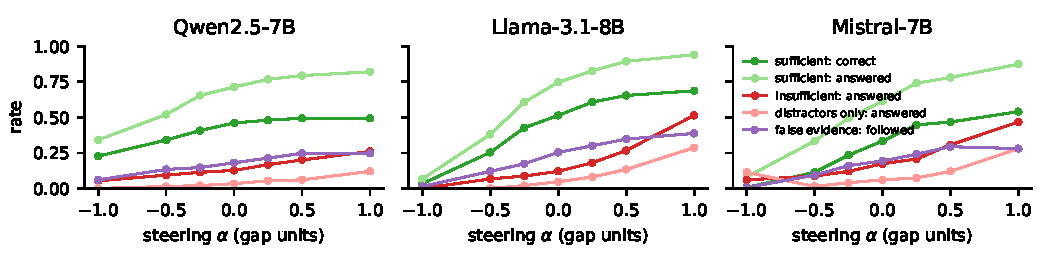
\includegraphics[width=0.84\linewidth]{steer_dose_response}
\caption{Dose-response of difference-of-means steering (four layers from the best sufficiency layer, from the anchor onward; $\alpha$ in units of the sufficient-minus-insufficient gap). Negative $\alpha$ induces abstention everywhere; positive $\alpha$ induces answering everywhere, including on distractors and false evidence.}
\label{fig:steer}
\end{figure*}

\section{Generalisation across models, datasets and evidence sources}
\label{sec:external}

\Cref{tab:probes} already shows the readouts in three model families, each with its own probes. This section asks whether the directions depend on \musique{}'s construction, on curated Wikipedia paragraphs, or on the stateless protocol in which every context is processed afresh.

\paragraph{Other protocols and datasets, without retraining.}
Applied unchanged, the 2-hop \musique{} directions reach $0.79$ (sufficiency) and $0.78$ (uptake) in a conversational protocol in which the model sees its previous answer before the new paragraph and is told to change it only if the evidence warrants it, so the transition is not an artefact of the stateless design. On \twowiki{} the sufficiency direction reaches $0.96$ ($0.93$ against matched controls) and uptake $0.79$, against $0.99$ and $0.91$ for probes trained on \twowiki{} itself. On 3--4-hop \musique{} questions sufficiency transfers at $0.82$--$0.85$; probes trained there reach $0.93$ on every split, while their uptake readout is less stable across splits ($0.61$--$0.80$). Details are in \cref{app:transfer,app:conversational,app:twowiki,app:multihop}.

\paragraph{External benchmarks.}
We then repeat the whole pipeline, unchanged and with Qwen2.5-7B, on HotpotQA, RAGBench and the synthetic benchmark (\cref{tab:external}). Sufficiency is decodable on every source ($0.98$, $0.90$, $0.97$) and against matched controls ($0.96$, $0.94$, $0.95$); on the synthetic data these controls include paraphrased duplicates, partial evidence and contradictions, and the increments are ordered along the direction as on \musique{}. Uptake is decodable on all three ($0.73$, $0.69$, $0.93$). It is not an artefact of multi-hop questions: it reaches $0.70$ on RAGBench single-hop questions, $0.79$ on HotpotQA comparison questions, whose two facts are independent lookups, and $0.99$ on single-hop synthetic questions, and it is above chance in every RAGBench domain ($0.56$--$0.78$; \cref{app:groups}). On HotpotQA, where we keep questions the model can answer without evidence, sufficiency is decoded equally well whether the model knows the answer closed-book or not ($0.984$ against $0.978$), so the readout is not a signal that the model ``needs'' evidence it lacks.

\begin{table*}[t]
\centering\scriptsize
\setlength{\tabcolsep}{2.5pt}
\begin{tabular}{lcccccccccccc}
\toprule
& \multicolumn{4}{c}{within-dataset probes (AUROC)} & \multicolumn{2}{c}{MuSiQue dir.} & \multicolumn{4}{c}{patched insufficient (answered)} & \multicolumn{2}{c}{proj.-out (answered)} \\
\cmidrule(lr){2-5}\cmidrule(lr){6-7}\cmidrule(lr){8-11}\cmidrule(lr){12-13}
Dataset & suff. & matched & uptake & corr. & suff. & uptake & none & full & $\parallel v$ & $\perp v$ & $\vdm$ & random \\
\midrule
HotpotQA & 0.979 & 0.961 & 0.729 & 0.846 & 0.952 & 0.649 & 0.41 & 0.92 & 0.41 & 0.92 & 0.17 & 0.92 \\
RAGBench & 0.898 & 0.944 & 0.685 & 0.742 & 0.706 & 0.550 & 0.15 & 0.72 & 0.15 & 0.72 & 0.10 & 0.73 \\
RAGBench (held-out sub-datasets) & 0.717 & 0.872 & 0.596 & 0.719 & 0.706 & 0.550 & -- & -- & -- & -- & -- & -- \\
Synthetic & 0.965 & 0.948 & 0.930 & 0.925 & 0.739 & 0.722 & 0.03 & 0.89 & 0.03 & 0.89 & 0.00 & 0.99 \\
Synthetic (held-out relation chains) & 0.945 & 0.925 & 0.883 & 0.897 & 0.739 & 0.722 & -- & -- & -- & -- & -- & -- \\
\bottomrule
\end{tabular}
\caption{External benchmarks (Qwen2.5-7B). Within-dataset probes trained and tested on the row's dataset; \musique{} 2-hop directions applied without retraining; and the patching and projection-out tests of \cref{sec:causal} (answered rate, 150 held-out questions). ``Held-out sub-datasets'' and ``held-out relation chains'' test on groups never seen in training.}
\label{tab:external}
\end{table*}

\paragraph{Transfer across construction and domain.}
The \musique{} directions transfer to HotpotQA at $0.95$ for sufficiency, but only partially to RAGBench ($0.71$; matched $0.78$; uptake $0.55$) and to the synthetic data ($0.74$; uptake $0.72$). Within RAGBench, holding out whole sub-datasets at test time drops sufficiency from $0.90$ to $0.72$ and uptake from $0.69$ to $0.60$; holding out relation chains on the synthetic data costs two to five points. The state is present under natural retrieval and in every domain, but its direction is partly dataset-specific: a detector trained on Wikipedia should not be deployed on biomedical or technical RAG without adaptation. The causal picture of \cref{sec:causal} replicates on all three sources: the full anchor patch makes the insufficient prompt answer ($0.41\to0.92$, $0.15\to0.72$, $0.03\to0.89$), the component along the probe direction does nothing, and projecting out $\vdm$ silences answering ($0.17$, $0.10$, $0.00$).

\paragraph{Retrieved and rewritten evidence.}
In a real RAG system the evidence comes from a retriever, not from a benchmark's curated paragraphs. We therefore rebuild the trajectories of 1{,}200 \musique{} questions with passages retrieved from the 21M-passage Wikipedia corpus distributed with FlashRAG \cite{jin2025flashrag,karpukhin2020dense}, by BM25 \cite{robertson2009bm25} or by the dense retriever E5 \cite{wang2022e5}, either keeping the gold paragraphs and retrieving all distractors, or retrieving all the evidence, which is possible for the 402 (E5) and 219 (BM25) questions for which retrieval found every hop. A further run varies the wording of the decisive paragraph with LLM paraphrases, value-withheld versions and paragraphs on the same entity written independently for HotpotQA or \twowiki{}. Nothing changes qualitatively (\cref{tab:estb}; construction and full results in \cref{app:estb}). Sufficiency stays at $0.91$--$0.95$, the \musique{} directions transfer at $0.91$--$0.94$ (sufficiency) and $0.76$--$0.82$ (uptake) on questions the source probes never saw, and the causal dissociation reproduces in every setting. Paraphrased and independently written decisive paragraphs project like the originals; partial and contradictory versions are the hardest controls, separated from decisive increments at only $0.81$ and $0.76$.

\section{Conclusion}
We asked whether a language model's internal state shows that newly retrieved evidence has become sufficient, and whether the model will use it. Both are readable from the residual stream at the answer position before generation, in three model families and under splits that keep documents, answers and relations disjoint. For sufficiency the internal state is a far better judge than the model's own output, which declares complete evidence insufficient a third of the time, and somewhat better than a text classifier given the whole context. For uptake, text alone says almost nothing, the model's decision to answer says much, and the internal state adds to it. The directions that carry these readouts are not the ones the model acts on; the only causal direction we found is a gate on abstention. The readouts transfer across datasets, fully to HotpotQA and partially to other domains and to retrieved evidence. Beyond what they say about the model, these readouts have practical uses: read before generation, the sufficiency score can decide when an adaptive retrieval system should stop fetching evidence, and the uptake score whether to trust the answer it then gives (\cref{app:adaptive}). We release the trajectory construction, the probing and intervention code, and the benchmark.

\section*{Limitations}
Our main experiments use questions the models cannot answer without evidence, under an instruction that asks for INSUFFICIENT when the evidence is lacking; the verbalised baseline depends on that instruction, while the internal readout changes little without it (\cref{app:augmented}). The uptake probe reads much of the model's decision to answer, and its advantage over output confidence among answered increments is small. The causal experiments on the external sources use Qwen only, RAGBench correctness relies on an LLM judge, and directions learned on Wikipedia transfer only partially to other domains. We tested additive, patching and projection interventions at the anchor position only.

% \section{Discussion}
\label{sec:discussion}

\paragraph{Two readable signals and one causal gate.}
Our results separate three things that the phrase ``an internal state transition'' tends to conflate. \emph{Sufficiency} is a property of the input: whether the context now contains every fact the question needs. The model represents it cleanly, but a text classifier that sees the same context can compute it too, and its causal counterpart in the model is an abstention gate. \emph{Uptake} is a property of the model: whether the same decisive paragraph will actually be used in the answer. It is predictable from activations but not from text, at $0.78$ AUROC across three model families and on every external source. Neither readout direction is a lever that controls the behaviour it predicts. What turns an insufficient state into an answer is high-dimensional, orthogonal to both readout directions, and on some models concentrated on the answer's unembedding direction. The picture is therefore a low-dimensional gate that decides whether to answer, plus high-dimensional content that determines the answer, rather than a single direction along which the model takes up new evidence.

\paragraph{Why probes do not find the lever, and what to use instead.}
A logistic probe looks for the direction along which the two classes are best separated relative to their spread. It therefore down-weights directions along which activations vary a lot within each class. The difference-of-means direction, in contrast, follows the raw shift between the class averages, and much of that shift lies along a high-variance axis related to answering. The projection-out and subspace experiments show that the causal content lies exactly there. A probe direction can thus score a high AUROC and transfer well across datasets while being causally irrelevant. Any proposed steering direction should therefore be validated with controls of the kind used here: projecting the direction out, measuring how many dimensions the effect needs, and comparing with random directions of matched norm. For retrieval systems, the most useful signal is uptake, as a detector of evidence the model has ignored. Sufficiency is tracked about as well by the model's own abstentions, and the abstention gate trades abstention against compliance uniformly rather than making the model more sensitive to the evidence.
   % kept for reviewers' questions on why probe directions are not levers

\bibliography{references}

\appendix
\section{Evidence conditions and increments}
\label{app:conditions}
This appendix lists every context (\emph{condition}) shown to the model for one question, and every pair of conditions (\emph{increment}) on which probes are trained. Consider a question with $n$ gold paragraphs $g_0,\dots,g_{n-1}$, one per reasoning hop, in the order given by the dataset's decomposition of the question, together with its pool of distractor paragraphs. The conditions are:
\begin{itemize}
  \item \textbf{Empty and distractor-only contexts.} $C_0$ contains no evidence. $C_D$ contains $n$ distractors, each matched in word count to one gold paragraph.
  \item \textbf{Chains.} Gold paragraphs are added one at a time, in the canonical hop order, in the reverse order and, for $n\ge3$, in random orders. Each chain gives the prefixes $C_{o_{1}},C_{o_{1}o_{2}},\dots$, and its last prefix is the minimal sufficient context. Each new paragraph is inserted at a uniformly random position among the paragraphs already present, so that the position of the decisive paragraph carries no information. Identical contexts reached through different orders are stored once.
  \item \textbf{Leave-one-out contexts} ($n\ge3$): all gold paragraphs but one, shuffled, followed by their completion with the missing paragraph.
  \item \textbf{Matched controls.} From every \emph{penultimate} context $S$, i.e.\ a chain or leave-one-out context that lacks exactly one gold paragraph, we build four controls alongside the decisive completion:
  $S{+}D$ adds a distractor matched in length to the missing paragraph;
  $S{+}R$ adds a verbatim duplicate of a gold paragraph already in $S$;
  $S{+}F$ adds the missing paragraph with its sub-answer (and title, if applicable) replaced by another question's sub-answer for the same relation, so the false paragraph remains plausible in type (questions whose sub-answer does not appear in the paragraph have no such control);
  $S{+}A$ adds a distractor with the sentence ``(Not to be confused with \{answer\}.)'' appended, so the answer string is present without the supporting fact.
  \item \textbf{Post-sufficiency contexts.} The canonical minimal sufficient context plus a distractor, plus a duplicate gold paragraph, or plus a falsified copy of the final hop that conflicts with it; and the full context of all 20 paragraphs, shuffled.
\end{itemize}
For 2-hop questions this gives 17 conditions and 17 increments per question. \Cref{tab:kinds} names the kinds of increment, as they appear in the tables and figures, groups them into the three families used in the main text (decisive, non-decisive, irrelevant), and shows which task uses each kind as a positive ($+$), as a negative ($-$) or not at all ($\cdot$). For uptake the label is behavioural ($\pm$: positive if the answer becomes correct). The conversational protocol (\cref{app:conversational}) re-runs the 10 chain-related increment kinds with the model's own stateless answer shown in the prompt (30{,}000 increments for Qwen).

\begin{table*}[t]
\centering\small
\setlength{\tabcolsep}{4pt}
\begin{tabular}{llp{7.2cm}ccc}
\toprule
Family & Kind & What the increment adds & Suff. & Matched & Uptake \\
\midrule
decisive & \texttt{decisive} & the last missing gold paragraph of a chain & $+$ & $+$ & $\pm$ \\
decisive & \texttt{loo\_decisive} & the missing gold paragraph of a leave-one-out context ($n\ge3$) & $+$ & $+$ & $\pm$ \\
non-decisive & \texttt{gold\_nondecisive} & a gold paragraph that still leaves another one missing & $-$ & $\cdot$ & $\cdot$ \\
irrelevant & \texttt{distractor\_from\_none} & distractors added to the empty context & $-$ & $\cdot$ & $\cdot$ \\
irrelevant & \texttt{distractor} & a length-matched distractor added to a penultimate context ($S{+}D$) & $-$ & $-$ & $\cdot$ \\
irrelevant & \texttt{redundant} & a duplicate of a gold paragraph already present ($S{+}R$) & $-$ & $-$ & $\cdot$ \\
irrelevant & \texttt{false} & the missing paragraph with a substituted sub-answer ($S{+}F$) & $-$ & $-$ & $\cdot$ \\
irrelevant & \texttt{answer\_ctrl} & a distractor that mentions the answer string ($S{+}A$) & $-$ & $-$ & $\cdot$ \\
irrelevant & \texttt{post\_distractor} & a distractor added to the minimal sufficient context & $-$ & $\cdot$ & $\cdot$ \\
irrelevant & \texttt{post\_redundant} & a duplicate gold paragraph added to the minimal sufficient context & $-$ & $\cdot$ & $\cdot$ \\
irrelevant & \texttt{post\_false} & a falsified copy of the final hop, conflicting with it, added to the minimal sufficient context & $-$ & $\cdot$ & $\cdot$ \\
irrelevant & \texttt{full\_context} & all remaining paragraphs added to the minimal sufficient context & $-$ & $\cdot$ & $\cdot$ \\
\bottomrule
\end{tabular}
\caption{Kinds of increment, their family, and their role in each task: positive ($+$), negative ($-$), unused ($\cdot$), or labelled by the model's behaviour ($\pm$). The sufficiency label $y^{\mathrm{suff}}$ is 1 exactly for the decisive family.}
\label{tab:kinds}
\end{table*}

\section{Probing, nuisance and intervention details}
\label{app:probing}
\paragraph{Activation capture.} Activations are read at the anchor position by forward hooks on the output of each decoder block. Prompts are processed in batches, left-padded so that the anchor has the same index in every row. In the same forward pass we append the gold answer tokens after the anchor. Because attention is causal, this leaves the anchor's activations unaffected, but it gives the log-probability the model assigns to the gold answer, which we use as a nuisance covariate. The cached keys and values are then cut back to the prompt, and the model decodes greedily from there. Layer index $l$ denotes the residual stream after block $l$ ($l=0$: embeddings).

\paragraph{Probes.} Probes are \texttt{scikit-learn} logistic regressions with L2 regularisation ($C=0.5$) and balanced class weights, on features standardised on the training split \cite{alain2016probes}; the layer is selected by grouped 3-fold cross-validation on training questions (never on test), and the reported number is the test AUROC at that layer. The probe direction is the weight vector $w$ divided by the per-feature standard deviations $\sigma$, so that it lives in the original activation space, and normalised to unit norm. The difference-of-means direction is the normalised difference of class means of $\Delta h$ (or of $h$ for state tasks). Bootstrap intervals resample test questions (1{,}000 draws) using the stored probe weights.

\paragraph{State probes.} State probes use the stored anchor activation of each condition, one example per condition, with the same estimator, standardisation, layer selection and question-level splits as the update probes. For a two-hop question the state-sufficiency task has five positive conditions: the minimal sufficient context in each hop order (de-duplicated when identical), sufficient plus a distractor, sufficient plus a duplicate, and the full context. It has ten negative ones: no evidence, distractors only, each single hop, and each penultimate state plus a distractor, a duplicate or an answer-string control. Conditions containing a falsified paragraph are excluded. All positives except the minimal sufficient context contain three or more paragraphs, and no negative does, so the task is partly separable by paragraph count; \cref{app:behaviour} reports a count-matched version restricted to two-paragraph contexts. State-correctness and abstention-flag probes use every condition, labelled by the model's own answer.

\paragraph{Nuisance covariates.} $\Delta$tokens, total tokens, $\Delta$ gold log-probability, $\Delta$ next-token entropy, $\Delta$ top probability, answer string in added text / in the full context / in the previous context, TF-IDF cosine relevance of the added passage to the question, number and word count of added paragraphs, relative insertion position, and a 16-dimensional truncated-SVD embedding of the added text's TF-IDF vector (fit on training increments). The nuisance-only classifier is a logistic regression on these covariates. The residualised probe first regresses $\Delta h$ on the covariates with ridge regression ($\lambda=1$) and then probes what the covariates do not explain. The ``gain'' is the AUROC added when out-of-fold probe scores (5-fold, grouped by question) are given to the nuisance classifier as an extra feature.

\paragraph{Text baselines.} TF-IDF (1--2-grams, sublinear tf, $\le200$k features) with logistic regression; DeBERTa-v3-base fine-tuned with AdamW (lr $3{\times}10^{-5}$, linear decay, class-weighted cross-entropy). The reduced budget uses one epoch, 256 tokens and 8{,}000 training increments (all positives kept); the full budget two epochs, 512 tokens and all training increments.

\paragraph{Interventions.} Steering adds the vector $\alpha\,u\,v$ at the anchor and every generated position (``anchor onward'') or at all positions; the unit $u$ is $|\mathbb E[v^\top h\mid\text{sufficient}]-\mathbb E[v^\top h\mid\text{insufficient}]|$ on training conditions, computed per layer, so that $\alpha=1$ moves the activation by one gap between the two class means. Projection-out sets $v^\top h$ to the insufficient-state mean at the anchor and generated positions for every layer from the best layer onward. Patching replaces the anchor residual during the prefill at every layer from the best layer to the last; decoding then proceeds from the patched cache. Principal components are computed from 1{,}500 training decisive updates per layer; the ``unembedding'' direction is the normalised row of the output embedding matrix for the gold answer's first token.

\section{Readout details: layer depth and projections by increment kind}
\label{app:readout}

\paragraph{Layer depth.}
Every probe in the paper is fitted at every layer, and the main text reports the layer selected by grouped cross-validation on the training questions. \Cref{fig:layers} shows the full profile. Sufficiency is readable from early layers and peaks at 50--60\% of the network's depth in all three models (layer 17 of 28 for Qwen), after which it declines slowly. Uptake and correction emerge later and peak near the end of the network (layer 26 of 28 for Qwen), which is where the content that determines the answer is assembled. The matched sufficiency task follows the sufficiency profile a few points lower. The same picture holds on the question, answer and relation splits.

\begin{figure*}[t]
\centering
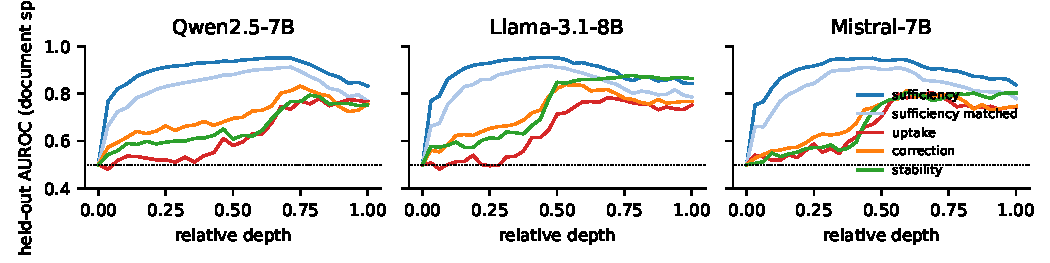
\includegraphics[width=0.84\linewidth]{auroc_by_layer}
\caption{Held-out AUROC by relative depth for the update tasks (document split). Sufficiency peaks around mid-depth in every model; uptake and correction emerge later.}
\label{fig:layers}
\end{figure*}

\paragraph{Projections by increment kind.}
\Cref{fig:kinds} projects every held-out increment onto the sufficiency direction, that is, it computes its score along the probe's weight vector, and averages by kind of increment. The kinds are ordered as one would expect if the direction encoded ``the evidence has just become complete'': decisive $>$ falsified $>$ distractor $>$ duplicate $>$ answer-string control $>$ a gold paragraph that does not yet complete the evidence. Increments added after the context is already sufficient, and the first hop added to an empty context, score far below. That the falsified paragraph scores second indicates that the direction encodes ``the final slot has been filled'' rather than truth, which is all the model can register before it generates; the behavioural counterpart is that a falsified final paragraph halves abstention (\cref{app:behaviour}).

\begin{figure}[t]
\centering
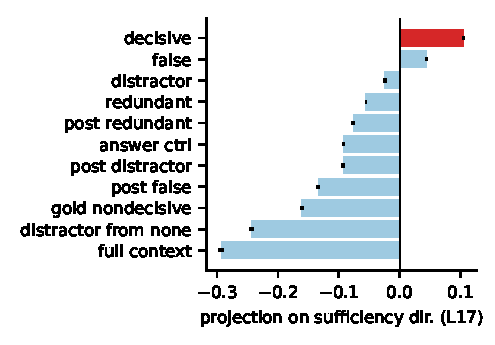
\includegraphics[width=\linewidth]{projection_by_kind}
\caption{Mean projection of held-out increments on the sufficiency direction, by kind of increment (Qwen2.5-7B, document split; standard errors). Red: decisive.}
\label{fig:kinds}
\end{figure}

\section{Related transitions: correction, stability and revision}
\label{app:related}

Sufficiency and uptake are the two properties the paper is about, but every increment carries the model's full behavioural transition, and this lets us probe three related properties with the same machinery. \emph{Correction} is defined on increments that start from a wrong or abstaining answer and asks whether the answer becomes correct; unlike uptake it includes non-decisive increments, so a correct answer may also come from guessing a hop or from a falsified paragraph. \emph{Stability} is defined on increments that start from a correct answer and asks whether it stays correct. \emph{Revision} is defined on all increments and asks whether the answer changes at all. \Cref{tab:probes_full} gives the probe results alongside those of the main text.

\begin{table*}[t]
\centering\scriptsize
\setlength{\tabcolsep}{3pt}
\begin{tabular}{lccccccccc}
\toprule
& \multicolumn{3}{c}{Qwen2.5-7B} & \multicolumn{3}{c}{Llama-3.1-8B} & \multicolumn{3}{c}{Mistral-7B} \\
\cmidrule(lr){2-4}\cmidrule(lr){5-7}\cmidrule(lr){8-10}
Task & AUROC [95\% CI] & nuis. & gain & AUROC [95\% CI] & nuis. & gain & AUROC [95\% CI] & nuis. & gain \\
\midrule
Sufficiency & 0.948 [0.94,0.95] & 0.87 & 0.11 & 0.952 [0.95,0.96] & 0.86 & 0.12 & 0.949 [0.94,0.95] & 0.87 & 0.11 \\
Sufficiency (matched) & 0.911 [0.90,0.92] & 0.90 & 0.07 & 0.918 [0.91,0.93] & 0.89 & 0.08 & 0.910 [0.90,0.92] & 0.90 & 0.07 \\
Uptake & 0.775 [0.74,0.80] & 0.66 & 0.14 & 0.783 [0.75,0.81] & 0.58 & 0.21 & 0.771 [0.74,0.80] & 0.59 & 0.18 \\
Correction & 0.730 [0.70,0.76] & 0.81 & 0.01 & 0.817 [0.79,0.84] & 0.83 & 0.06 & 0.792 [0.77,0.81] & 0.85 & 0.03 \\
Stability & 0.750 [0.72,0.78] & 0.92 & $-$0.01 & 0.869 [0.85,0.89] & 0.90 & 0.02 & 0.800 [0.77,0.83] & 0.90 & 0.01 \\
\bottomrule
\end{tabular}
\caption{Held-out AUROC of the best-layer probe on paired updates for all five tasks (document split; 95\% question-level bootstrap intervals), with the nuisance-only AUROC and the gain from adding the probe score to the nuisance classifier.}
\label{tab:probes_full}
\end{table*}

\paragraph{Results.} Correction is readable at $0.73$--$0.82$ and stability at $0.75$--$0.87$, but both are largely explained by surface properties, chiefly the change in the model's output distribution: the nuisance-only classifier reaches $0.81$--$0.85$ on correction and $0.90$--$0.92$ on stability, and the probe adds at most $0.06$. Revision is readable at $0.71$--$0.77$ (\cref{tab:rep_ablation}). The model's own output is an even stronger predictor of these three: whether the model answers after the increment predicts correction at $0.88$--$0.90$ and stability at $0.80$--$0.90$, because a corrected answer is by definition an answer and a destabilised one is often an abstention. These tasks are therefore less informative about the internal state than uptake, which is the one task on which the activations add far more than surface properties or the output.

\paragraph{Cross-task transfer.} \Cref{fig:transfer} applies the direction learned for one task (row) to the increments of another (column), at the row task's best layer, on the test questions of the document split. Uptake and correction share a direction: the cosine between them is $0.30$--$0.34$, and each predicts the other task at $0.82$. Both are nearly orthogonal to sufficiency (cosine $0.02$--$0.03$), whose direction reaches only $0.54$--$0.60$ on uptake. Stability and revision form a third group, aligned with the change in output distribution.

\begin{figure}[t]
\centering
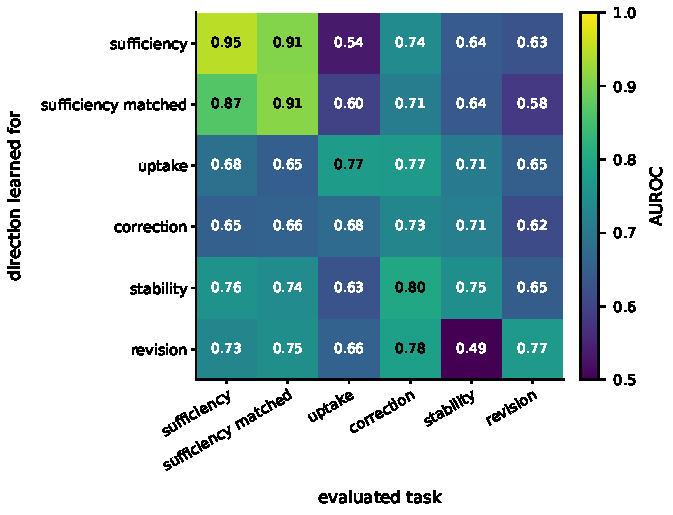
\includegraphics[width=\linewidth]{transfer_matrix}
\caption{Cross-task transfer (Qwen2.5-7B, document split): AUROC of the direction learned for the row task, evaluated on the column task.}
\label{fig:transfer}
\end{figure}

\section{State versus update: which representation carries the readout?}
\label{app:rep}

The probes of \cref{tab:probes} act on the paired update $\Delta h=h(C_k)-h(C_{k-1})$. A natural question is how much of their accuracy comes from the \emph{change} of state, and how much from information already present in either absolute state. If $h(C_k)$ alone did as well, the finding would be that the model's current state represents whether its evidence is sufficient. If $h(C_k)$ were much worse than $\Delta h$, sufficiency would be encoded specifically in the transition caused by the new evidence.

\paragraph{Protocol.} For every update task we refit the probe on four representations of the \emph{same} increments, with the same labels, document split, regularisation ($C=0.5$, balanced classes) and layer selection (grouped three-fold cross-validation on training questions, over all blocks):
\begin{itemize}
  \item $h(C_{k-1})$, the anchor state before the new evidence;
  \item $h(C_k)$, the anchor state after it;
  \item $\Delta h$, the paper's representation (it reproduces \cref{tab:probes} to within $0.002$);
  \item the concatenation $[h(C_{k-1});h(C_k)]$, from which a linear probe can represent $\Delta h$, either state, or any other linear combination of the two.
\end{itemize}
Both states are the stored activations of the two stateless forward passes; $\Delta h$ is their difference to within float16 precision.

\begin{table*}[t]
\centering\small
\begin{tabular}{llcccc}
\toprule
Model & Task & $h(C_{k-1})$ & $h(C_k)$ & $\Delta h$ & $[h(C_{k-1});h(C_k)]$ \\
\midrule
Qwen2.5-7B & Sufficiency & 0.733 & 0.930 & 0.947 & \textbf{0.949} \\
 & Sufficiency (matched) & 0.500 & 0.901 & 0.911 & \textbf{0.919} \\
 & Uptake & 0.605 & \textbf{0.798} & 0.775 & 0.780 \\
 & Correction & 0.574 & 0.766 & 0.730 & \textbf{0.782} \\
 & Stability & 0.549 & 0.813 & 0.750 & \textbf{0.832} \\
 & Revision & 0.556 & \textbf{0.806} & 0.767 & 0.791 \\
\midrule
Llama-3.1-8B & Sufficiency & 0.733 & 0.936 & \textbf{0.952} & 0.950 \\
 & Sufficiency (matched) & 0.500 & 0.908 & 0.917 & \textbf{0.923} \\
 & Uptake & 0.570 & \textbf{0.794} & 0.783 & 0.788 \\
 & Correction & 0.522 & 0.872 & 0.818 & \textbf{0.883} \\
 & Stability & 0.592 & 0.882 & 0.869 & \textbf{0.888} \\
 & Revision & 0.563 & \textbf{0.795} & 0.709 & 0.751 \\
\midrule
Mistral-7B & Sufficiency & 0.733 & 0.940 & 0.948 & \textbf{0.949} \\
 & Sufficiency (matched) & 0.500 & 0.900 & \textbf{0.910} & 0.907 \\
 & Uptake & 0.647 & 0.769 & 0.771 & \textbf{0.775} \\
 & Correction & 0.566 & \textbf{0.822} & 0.790 & 0.819 \\
 & Stability & 0.524 & \textbf{0.857} & 0.800 & 0.857 \\
 & Revision & 0.634 & 0.789 & 0.721 & \textbf{0.790} \\
\bottomrule
\end{tabular}
\caption{Held-out AUROC (document split, best layer by inner cross-validation) of probes for each update task, fitted on four representations of the same increments. Bold: best per row.}
\label{tab:rep_ablation}
\end{table*}

\paragraph{Sufficiency.} The state \emph{after} the new evidence carries most of the readout. $h(C_k)$ reaches $0.930$--$0.940$ on the full task and $0.900$--$0.908$ on the matched one, against $0.947$--$0.952$ and $0.910$--$0.917$ for $\Delta h$. The state \emph{before} the evidence is uninformative beyond the trajectory stage. On the full task it scores $0.733$ in all three models, which is exactly the AUROC of an oracle that knows only whether the increment starts from the empty context, a partial context or an already sufficient one: $20\%$ of increments starting from a partial context are decisive, and none of the others. On the matched task, where the decisive increment and its four controls start from the same state, it scores exactly $0.500$. The concatenation matches $\Delta h$ ($0.949$--$0.950$; matched $0.907$--$0.923$). So subtracting the earlier state adds no information that having both states does not; what it does is remove the large question-specific component that both states share, which makes a single linear direction work.

\paragraph{Why $h(C_k)$ is not trivially enough.} On the full task, $27\%$ of negatives end in a context that is already sufficient: a distractor, duplicate or falsified paragraph added after sufficiency, or the full context. A pure ``is this context sufficient?'' detector cannot reject them. Applying the state-sufficiency probe of \cref{tab:probes} (trained on whole contexts, $0.99$ AUROC on its own task) to $h(C_k)$ of these increments gives only $0.70$ on the full update task, and $0.87$--$0.90$ on the matched task, where no negative ends in a sufficient context. The $h(C_k)$ probe can, because the state after the decisive paragraph differs from the state after a post-sufficiency addition: the former is a \emph{minimal} sufficient context, the latter has more paragraphs. Part of what separates them is plausibly context size. On the matched task this cannot help, because every control adds exactly one paragraph to the same penultimate state. There, $h(C_k)$ at $0.90$ is a genuine readout of sufficiency from the resulting state.

\paragraph{Uptake, correction, stability, revision.} For the behavioural tasks the state after the evidence is as informative as the update or more so: uptake $0.769$--$0.798$ against $0.771$--$0.783$, correction $0.766$--$0.872$ against $0.730$--$0.818$, stability $0.813$--$0.882$ against $0.750$--$0.869$, revision $0.789$--$0.806$ against $0.709$--$0.767$. The concatenation is best or tied on most of them. The earlier state carries a little information of its own here ($0.52$--$0.65$): how the model behaves after new evidence depends partly on the state it was in. These tasks are about the model's \emph{resulting} answer, so it is unsurprising that the resulting state predicts them best. The uptake result means the signal that decisive evidence will be integrated is present in the state after the evidence arrives, before generation, and does not require comparing with the state before it.

\paragraph{What this means for the paper's claims.}
\begin{itemize}
  \item The informational claims stand: sufficiency and uptake are linearly readable at the answer-start position before generation, robustly across splits and models. But ``readable from the update'' should be understood as ``readable from the resulting state, measured in a design that controls for the starting state''. The paired update is the cleanest way to read the state change without question-specific content, and it is what makes the matched controls possible (same starting state). It is not the source of the information.
  \item The causal analysis of \cref{sec:causal} is unaffected. It patches the anchor residual of the insufficient prompt with that of the sufficient prompt, which is the same as adding $\Delta h$ to $h(C_{k-1})$. Its conclusion, that the probe direction is inert while the full residual and $\vdm$ are causal, concerns directions in this space whichever way they were found.
  \item The text-baseline comparison (\cref{sec:text}) is unaffected: it compares classifiers on the same increments and labels.
\end{itemize}

\section{Behaviour, verbalised sufficiency and the internal state}
\label{app:behaviour}

This appendix does three things. It describes how the models behave on each condition family, which supplies the behavioural labels behind uptake, correction, stability and revision. It shows that the model's own output, read as a judgement about whether the evidence is sufficient, is frequently wrong. And it shows that the sufficiency state read from the residual stream at the same position, in the same forward pass, is a much more accurate signal than that verbalised judgement, including in the cases where the verbalised judgement is wrong.

\subsection{Behaviour by condition family}

\Cref{tab:behaviour} reports, for every condition family of \cref{app:conditions}, the fraction of greedy answers that are correct and the fraction that are INSUFFICIENT. It covers the evidence-only regime over the 2{,}000 two-hop questions of each model. The remaining fraction is a wrong answer. All questions are ones the model answers incorrectly closed-book (\cref{sec:setup}), so a correct answer can be attributed to the evidence.

\begin{table*}[t]
\centering\small
\begin{tabular}{lccc}
\toprule
Condition (correct / abstain) & Qwen2.5-7B & Llama-3.1-8B & Mistral-7B \\
\midrule
no evidence & 0.00 / 1.00 & 0.00 / 1.00 & 0.00 / 0.99 \\
distractors only & 0.00 / 0.97 & 0.00 / 0.97 & 0.00 / 0.94 \\
one hop & 0.10 / 0.80 & 0.12 / 0.76 & 0.13 / 0.69 \\
minimal sufficient & 0.46 / 0.30 & 0.47 / 0.31 & 0.36 / 0.36 \\
one hop + false final hop & 0.13 / 0.49 & 0.13 / 0.55 & 0.12 / 0.51 \\
sufficient + distractor & 0.39 / 0.35 & 0.38 / 0.41 & 0.27 / 0.47 \\
full context (20 par.) & 0.22 / 0.38 & 0.17 / 0.61 & 0.17 / 0.48 \\
\bottomrule
\end{tabular}
\caption{Behaviour by condition family (evidence-only regime, 2{,}000 questions per model): fraction correct / fraction answering INSUFFICIENT. The remaining fraction is a wrong answer.}
\label{tab:behaviour}
\end{table*}

Read row by row:
\begin{itemize}
  \item \textbf{No evidence and distractors only.} The instruction is followed. The models almost never answer ($94$--$100\%$ INSUFFICIENT) and are never correct. With distractors alone, the $3$--$6\%$ of prompts that are answered are hallucinations.
  \item \textbf{One hop.} With only one of the two gold paragraphs, the evidence is insufficient by construction, yet the models answer $20$--$31\%$ of the time and are correct $10$--$13\%$ of the time. Some second hops can be guessed from the first, which is one reason correctness and sufficiency are separate labels.
  \item \textbf{Minimal sufficient.} With both gold paragraphs present and nothing else, the models answer correctly only $36$--$47\%$ of the time, and they say INSUFFICIENT $30$--$36\%$ of the time. The evidence is sufficient by construction: \musique{} composes each question from single-hop questions whose supporting paragraphs are exactly these gold paragraphs. An INSUFFICIENT output here is therefore a \emph{verbalised false negative}: the model declares the evidence insufficient when it is not. The remaining $22$--$28\%$ are wrong answers.
  \item \textbf{One hop plus a falsified final hop.} Replacing the decisive paragraph with a version whose sub-answer is swapped roughly halves abstention ($49$--$55\%$ INSUFFICIENT, against $69$--$80\%$ with one hop alone). The models treat a type-plausible but false final hop much as they treat the true one, which is what the sufficiency readout also does (\cref{sec:readout}: the false increment projects second only to the decisive one).
  \item \textbf{Sufficient plus a distractor, and the full context.} Adding irrelevant paragraphs to a sufficient context makes the models abstain \emph{more}: $35$--$47\%$ with one extra distractor and $38$--$61\%$ with all 20 paragraphs. Correctness falls accordingly ($0.17$--$0.39$). Verbalised sufficiency judgements degrade as the context grows, even though the evidence is unchanged.
\end{itemize}

\subsection{The verbalised judgement is a poor sufficiency detector; the internal state is a good one}

Because the prompt instructs the model to output INSUFFICIENT exactly when the evidence does not determine the answer, its output is a binary sufficiency judgement: \emph{answers} means ``judged sufficient'', \emph{INSUFFICIENT} means ``judged insufficient''. We compare this verbalised judgement with the state-sufficiency probe (\cref{sec:method}), which reads the residual stream at the answer-start anchor of the same forward pass, before any token is generated.

\paragraph{Protocol.} The comparison uses the held-out conditions of the document split, with conditions containing falsified evidence excluded, as in the probe task. These are about $2{,}700$ sufficient and $6{,}000$ insufficient contexts per model. For the verbalised judgement we report its true-positive rate (sufficient contexts answered), its false-positive rate (insufficient contexts answered) and its AUROC as a binary score. For the probe we report AUROC and two operating points, both with the threshold set on \emph{training} contexts. The first matches the false-positive rate of the verbalised judgement, so the probe raises false alarms on insufficient contexts as often as the model's own answers do. The second requires $0.95$ precision. At each operating point we report the probe's recall on the sufficient contexts the model wrongly called INSUFFICIENT (\emph{wrong abstentions}), and its false-alarm rate on the insufficient contexts the model correctly called INSUFFICIENT.

\paragraph{A confound, and how we remove it.} Every condition with three or more paragraphs is sufficient (sufficient plus a distractor, sufficient plus a duplicate, full context). Every insufficient condition has at most two. Paragraph count, and with it prompt length, therefore separates part of the state task on its own. This inflates the state probe's headline AUROC ($0.99$) and makes its recall on wrong abstentions in the three larger families trivially perfect. We therefore also report a \emph{paragraph-count-matched} version. It keeps only two-paragraph contexts: the minimal sufficient context against distractors only and the penultimate state plus a distractor, a duplicate or an answer-string control. The probe is retrained on these contexts alone, so neither count nor length can separate the classes. The count-matched numbers are the ones we interpret.

\begin{table*}[t]
\centering\scriptsize
\setlength{\tabcolsep}{3pt}
\begin{tabular}{lccc}
\toprule
 & Qwen2.5-7B & Llama-3.1-8B & Mistral-7B \\
\midrule
\multicolumn{4}{l}{\emph{Held-out contexts}} \\
\quad sufficient / insufficient & 2754 / 6090 & 2701 / 6000 & 2754 / 6100 \\
\quad sufficient but verbalised INSUFFICIENT & 901 (33\%) & 1079 (40\%) & 1183 (43\%) \\
\multicolumn{4}{l}{\emph{Verbalised judgement (answers = sufficient)}} \\
\quad AUROC & 0.762 & 0.722 & 0.681 \\
\quad TPR / FPR & 0.673 / 0.150 & 0.601 / 0.156 & 0.570 / 0.208 \\
\multicolumn{4}{l}{\emph{State-sufficiency probe at the same anchor}} \\
\quad AUROC & 0.992 & 0.994 & 0.996 \\
\quad TPR / FPR, threshold at verbalised FPR & 0.995 / 0.188 & 0.996 / 0.178 & 1.000 / 0.194 \\
\qquad recall on wrongly abstained sufficient contexts & 0.990 & 0.991 & 0.999 \\
\qquad false alarms on correctly abstained insufficient contexts & 0.154 & 0.151 & 0.167 \\
\quad TPR / FPR, threshold at 0.95 precision & 0.962 / 0.050 & 0.970 / 0.051 & 0.977 / 0.038 \\
\qquad recall on wrongly abstained sufficient contexts & 0.936 & 0.956 & 0.961 \\
\qquad false alarms on correctly abstained insufficient contexts & 0.039 & 0.040 & 0.029 \\
\multicolumn{4}{l}{\emph{Wrong abstentions by condition: abstain rate; probe recall at 0.95 precision}} \\
\quad minimal sufficient & 0.29; 0.79 & 0.30; 0.84 & 0.37; 0.87 \\
\quad sufficient + distractor & 0.35; 1.00 & 0.41; 1.00 & 0.49; 1.00 \\
\quad sufficient + duplicate & 0.29; 0.99 & 0.34; 0.99 & 0.39; 1.00 \\
\quad full context (20 par.) & 0.40; 1.00 & 0.60; 1.00 & 0.50; 1.00 \\
\multicolumn{4}{l}{\emph{Mean probe score (0 = insufficient mean, 1 = sufficient mean on training contexts)}} \\
\quad sufficient, answered & 0.98 & 0.88 & 0.95 \\
\quad sufficient, verbalised INSUFFICIENT & 1.03 & 1.15 & 1.04 \\
\quad insufficient, answered & 0.10 & 0.08 & 0.04 \\
\quad insufficient, verbalised INSUFFICIENT & -0.01 & -0.00 & -0.03 \\
\midrule
\multicolumn{4}{l}{\emph{Two-paragraph contexts only (paragraph count matched; probe retrained on them)}} \\
\quad minimal sufficient / insufficient two-paragraph & 927 / 4263 & 901 / 4200 & 924 / 4270 \\
\quad minimal sufficient but verbalised INSUFFICIENT & 268 & 273 & 341 \\
\quad verbalised judgement: AUROC; TPR / FPR & 0.774; 0.71 / 0.16 & 0.773; 0.70 / 0.15 & 0.711; 0.63 / 0.21 \\
\quad probe AUROC (all two-paragraph contexts) & 0.976 & 0.981 & 0.986 \\
\quad probe AUROC among contexts verbalised INSUFFICIENT & 0.967 & 0.972 & 0.982 \\
\quad threshold at verbalised FPR: TPR / FPR & 0.984 / 0.196 & 0.986 / 0.187 & 0.997 / 0.213 \\
\qquad recall on wrong abstentions; false alarms on correct abstentions & 0.963; 0.171 & 0.963; 0.161 & 0.991; 0.188 \\
\quad threshold at 0.95 precision: TPR / FPR & 0.859 / 0.041 & 0.890 / 0.047 & 0.905 / 0.039 \\
\qquad recall on wrong abstentions; false alarms on correct abstentions & 0.757; 0.032 & 0.773; 0.037 & 0.812; 0.028 \\
\quad mean probe score: sufficient answered / sufficient abstained & 1.03 / 0.82 & 1.03 / 0.80 & 1.03 / 0.87 \\
\quad mean probe score: insufficient answered / insufficient abstained & 0.16 / -0.01 & 0.14 / -0.01 & 0.08 / -0.04 \\
\bottomrule
\end{tabular}
\caption{Verbalised versus internal sufficiency judgements on held-out contexts (document split; falsified-evidence contexts excluded). Verbalised: the model answers (judged sufficient) or says INSUFFICIENT. Probe: state-sufficiency probe at the answer-start anchor of the same forward pass; thresholds are set on training contexts. ``Wrong abstentions'': sufficient contexts the model called INSUFFICIENT; ``correct abstentions'': insufficient contexts it called INSUFFICIENT. Mean probe scores are expressed so that $0$ is the mean of insufficient and $1$ the mean of sufficient training contexts. Top block: all contexts, inflated by paragraph count. Bottom block: two-paragraph contexts only, with the probe retrained on them.}
\label{tab:verbal_internal}
\end{table*}

\paragraph{Results (\cref{tab:verbal_internal}).}
\begin{itemize}
  \item \textbf{The verbalised judgement is wrong on a third or more of sufficient contexts.} On held-out data the models call $33\%$ (Qwen), $40\%$ (Llama) and $43\%$ (Mistral) of sufficient contexts INSUFFICIENT, while still answering $15$--$21\%$ of insufficient ones. As a sufficiency classifier the output reaches $0.76$, $0.72$ and $0.68$ AUROC ($0.77$, $0.77$, $0.71$ on two-paragraph contexts).
  \item \textbf{The internal state is far more accurate, with paragraph count held fixed.} On two-paragraph contexts the retrained probe separates minimal sufficient from insufficient contexts at $0.976$, $0.981$ and $0.986$ AUROC. This is $0.20$--$0.27$ above the verbalised judgement made in the same forward pass.
  \item \textbf{It is accurate precisely where the verbalised judgement fails.} Restricted to the two-paragraph contexts the model called INSUFFICIENT, so that the output is held fixed, the probe still separates the sufficient ones from the insufficient ones at $0.967$--$0.982$. At $0.95$ training precision it recovers $76\%$, $77\%$ and $81\%$ of the wrongly rejected minimal sufficient contexts, with $3$--$4\%$ false alarms on correctly rejected insufficient ones. At the verbalised false-alarm rate it recovers $96$--$99\%$ of them. In practical terms, a detector reading the anchor before generation would accept most of the complete evidence the model itself refuses, at a fraction of the false alarms the model's own answers produce.
  \item \textbf{But the internal state is weaker in exactly those cases.} In units where the insufficient training mean is $0$ and the sufficient one is $1$, wrongly rejected minimal sufficient contexts score $0.82$, $0.80$ and $0.87$, against $1.03$ for sufficient contexts the model answers. Insufficient contexts score about $0$ when rejected and $0.08$--$0.16$ when (wrongly) answered. The internal sufficiency state is graded. The verbal decision behaves like a thresholded and noisier read-out of it, which tends to fail when the state is weaker than usual, but the state in those cases is still much closer to ``sufficient'' than to ``insufficient''. (Without the count matching, the wrongly rejected contexts appear to score as high as answered ones, $1.03$--$1.15$. That impression comes from the larger, trivially separable families and should not be relied on.)
  \item \textbf{Adding paragraphs hurts the verbal judgement.} The abstention rate on sufficient contexts rises from $29$--$37\%$ (minimal) to $40$--$60\%$ (full context), while every wrongly rejected full-context prompt is still on the sufficient side of the probe's threshold. Paragraph count makes that last comparison easy, so we do not interpret it further.
\end{itemize}

\subsection{Holding the output fixed for the update probes}

The same question can be asked of the update probes of \cref{tab:probes}: is ``the evidence just became sufficient'' anything more than ``the model just switched from INSUFFICIENT to an answer''? \Cref{tab:behaviour_control} reports, for the sufficiency and matched-sufficiency tasks with $\Delta h$ and with $h(C_k)$ (\cref{app:rep}), and for the state-sufficiency task, four numbers:
\begin{itemize}
  \item the AUROC of the output alone: the indicator that the model answers at $C_k$ (for updates, the indicator that it switched from INSUFFICIENT to an answer scores within $0.04$ of this);
  \item the standard probe, trained on all increments, scored separately on the test increments after which the model \emph{still says INSUFFICIENT} and on those after which it answers (``stratified'');
  \item probes trained \emph{and} tested only within each of these two groups (``within''). Within the abstaining group, the positives are decisive increments that completed the evidence while the model went on refusing, and the negatives are controls after which it also refused.
\end{itemize}

\begin{table*}[t]
\centering\scriptsize
\setlength{\tabcolsep}{3pt}
\begin{tabular}{lllcccccc}
\toprule
& & & output & all & \multicolumn{2}{c}{model abstains at $C_k$} & \multicolumn{2}{c}{model answers at $C_k$} \\
\cmidrule(lr){6-7}\cmidrule(lr){8-9}
Model & Task & Repr. & only & test & stratified & within & stratified & within \\
\midrule
Qwen2.5-7B & Sufficiency & $\Delta h$ & 0.685 & 0.945 & 0.948 & 0.944 & 0.929 & 0.927 \\
 & Sufficiency & $h(C_k)$ & 0.685 & 0.930 & 0.930 & 0.918 & 0.904 & 0.890 \\
 & Matched & $\Delta h$ & 0.721 & 0.911 & 0.891 & 0.884 & 0.879 & 0.870 \\
 & Matched & $h(C_k)$ & 0.721 & 0.909 & 0.904 & 0.883 & 0.854 & 0.843 \\
 & State suff. & $h(C)$ & 0.762 & 0.992 & 0.990 & 0.982 & 0.986 & 0.983 \\
\midrule
Llama-3.1-8B & Sufficiency & $\Delta h$ & 0.692 & 0.950 & 0.940 & 0.935 & 0.942 & 0.929 \\
 & Sufficiency & $h(C_k)$ & 0.692 & 0.927 & 0.931 & 0.914 & 0.893 & 0.892 \\
 & Matched & $\Delta h$ & 0.726 & 0.912 & 0.896 & 0.883 & 0.875 & 0.855 \\
 & Matched & $h(C_k)$ & 0.726 & 0.908 & 0.908 & 0.886 & 0.840 & 0.838 \\
 & State suff. & $h(C)$ & 0.722 & 0.992 & 0.992 & 0.988 & 0.986 & 0.982 \\
\midrule
Mistral-7B & Sufficiency & $\Delta h$ & 0.646 & 0.948 & 0.949 & 0.937 & 0.939 & 0.931 \\
 & Sufficiency & $h(C_k)$ & 0.646 & 0.936 & 0.944 & 0.933 & 0.912 & 0.912 \\
 & Matched & $\Delta h$ & 0.671 & 0.910 & 0.918 & 0.887 & 0.874 & 0.876 \\
 & Matched & $h(C_k)$ & 0.671 & 0.902 & 0.909 & 0.872 & 0.860 & 0.856 \\
 & State suff. & $h(C)$ & 0.681 & 0.996 & 0.996 & 0.994 & 0.994 & 0.989 \\
\bottomrule
\end{tabular}
\caption{Sufficiency probes with the model's output held fixed (document split). Output only: AUROC of the indicator ``the model answers at $C_k$''. All: standard probe, all test increments. Stratified: the same probe on the test increments after which the model abstains (resp.\ answers). Within: probe trained and tested only on that group, layer re-selected by grouped inner cross-validation. The state-sufficiency rows are not count-matched (see \cref{tab:verbal_internal} for the count-matched version).}
\label{tab:behaviour_control}
\end{table*}

The output alone gives $0.65$--$0.76$. The probes lose almost nothing when the output is held fixed. Among increments after which the model still says INSUFFICIENT, the $\Delta h$ sufficiency probe scores $0.940$--$0.949$ (stratified) and $0.935$--$0.944$ (within), against $0.945$--$0.950$ overall; for $h(C_k)$ the corresponding figures are $0.930$--$0.944$ and $0.914$--$0.933$. Among increments after which the model answers, the probes score slightly lower ($0.929$--$0.942$ for $\Delta h$), because there the controls that the model answers (false evidence, answer-string controls) are the hardest ones. On the matched task, where every control starts from the same state as the decisive increment, the probes reach $0.883$--$0.887$ even when trained and tested only on increments the model refuses.

\subsection{What this does and does not show}

\begin{itemize}
  \item \textbf{The sufficiency readout is not the planned output.} If the probes were reading ``about to output INSUFFICIENT'', they would fall to chance once the output is held fixed. They stay at $0.88$--$0.99$ depending on the task. The residual stream at the answer-start position encodes that the context contains the complete evidence, separately from the decision to answer.
  \item \textbf{The internal signal is a better sufficiency detector than the model's self-report.} For a system that has to decide whether retrieved evidence is complete, the anchor activation, read before generation, is more accurate than asking the model and reading its answer: $0.98$ against $0.71$--$0.77$ AUROC with paragraph count matched. At $0.95$ precision the probe accepts $86$--$91\%$ of sufficient contexts with $4\%$ false alarms, whereas the model's answers accept $63$--$71\%$ with $15$--$21\%$ false alarms.
  \item \textbf{This is a statement about evidence completeness, not about the answer.} The probe is trained on construction labels (all gold hops present). A high score on a wrongly rejected context says that the representation registers the evidence as complete. It does not say that the model could compute the answer from it. Whether it will is what uptake measures (\cref{sec:readout}), and uptake is lower and nearly orthogonal to sufficiency. Among the minimal sufficient contexts it rejects, the model may lack the bridging step, and the internal sufficiency state cannot supply it. Consistently, using the sufficiency score to stop retrieval does not by itself improve accuracy (\cref{app:adaptive}): stopping at a sufficient context the model will not answer from still yields INSUFFICIENT.
  \item \textbf{The causal picture is consistent with this division.} The one causally active direction, $\vdm$, acts as an abstention gate (\cref{sec:causal}): pushing along it makes the model answer, including on some sufficient contexts it was rejecting (positive steering adds $3$ points of correct answers on Qwen and $18$ on Llama), but also on distractors and false evidence. The sufficiency \emph{readout} is not that gate: projecting the probe direction out changes nothing. The model represents completeness accurately along directions it does not use for the answer/abstain decision, and its decision is driven by a lower-dimensional, noisier gate.
  \item \textbf{Scope.} The comparison uses \musique{} two-hop questions the models answer incorrectly closed-book, under the evidence-only instruction. With a more permissive instruction (\cref{app:augmented}), the models abstain less on sufficient evidence and follow false evidence more, so the verbalised false-negative rate depends on the prompt; the internal update readout barely changes ($0.945$ against $0.948$).
\end{itemize}

\subsection{Uptake and the decision to answer}
\label{app:uptake-answer}
The same question can be asked of the uptake probe: how much of its $0.78$ AUROC is the model's own decision to answer? Uptake is positive when the decisive increment makes the answer correct, and a correct answer is by definition an answer, whereas $45$--$55\%$ of the decisive increments the model fails to take up are ones after which it says INSUFFICIENT. The indicator ``the model answers after the increment'' therefore reaches $0.78$ on its own, exactly the probe's AUROC (\cref{tab:baselines}). \Cref{tab:uptake_given} restricts the comparison to the decisive increments the model answers, where the only remaining question is whether the answer is right. Three internal or output signals are compared there: the output confidence (negative next-token entropy at the anchor; top-token probability gives the same numbers to within $0.005$), the stored uptake probe trained on all decisive increments, and a probe refitted on the answered increments only, at the stored best layer. The right-hand block combines each signal with the decision to answer, ranking abstentions below every answer and answers by the signal.

\begin{table*}[t]
\centering\small
\begin{tabular}{lrccccccc}
\toprule
& & & \multicolumn{3}{c}{answered increments only} & \multicolumn{3}{c}{all decisive increments} \\
\cmidrule(lr){4-6}\cmidrule(lr){7-9}
Model & $n$ & correct & confidence & probe & probe (refit) & verbalised & + confidence & + probe \\
\midrule
Qwen2.5-7B & 867 & 0.67 & 0.636 & 0.658 & 0.665 & 0.776 & 0.837 & 0.850 \\
Llama-3.1-8B & 833 & 0.66 & 0.632 & 0.651 & 0.678 & 0.783 & 0.840 & 0.860 \\
Mistral-7B & 778 & 0.53 & 0.638 & 0.629 & 0.638 & 0.775 & 0.837 & 0.837 \\
\bottomrule
\end{tabular}
\caption{Uptake among the decisive increments the model answers (document split, test questions). $n$: answered test increments; ``correct'': fraction correct among them. Left: AUROC for correct against wrong answers of output confidence, of the uptake probe trained on all decisive increments, and of a probe refitted on answered increments. Right: AUROC on all decisive increments of the decision to answer alone and combined with confidence or with the refitted probe.}
\label{tab:uptake_given}
\end{table*}

Among answered increments the probe separates correct from wrong answers at $0.63$--$0.68$ and confidence at $0.63$--$0.64$: the probe is ahead by $0.03$ on Qwen and $0.05$ on Llama and level on Mistral. Combined with the decision to answer, the probe reaches $0.84$--$0.86$ and confidence $0.84$. Two things follow. The uptake probe does carry information that the text does not have (no text classifier exceeds $0.60$) and that the model's output does not fully have, but the larger part of its $0.78$ is the decision to answer, which the model verbalises for free. And the part specific to correctness is modest and only a little better than the model's own confidence, so claims that internal states predict evidence uptake should be read with this decomposition in mind. The verification experiment of \cref{app:adaptive}, which uses the uptake direction to decide whether to trust the answer given once retrieval stops, measures the same quantity on a different set of contexts and reaches the same conclusion.

\section{Robustness across data splits}
\label{app:splits}
Every probe is trained on 70\% of questions and tested on the remaining 30\% under four groupings that are never shared between train and test: question id; gold document, where questions that share any supporting page are grouped together (transitively) and each group goes entirely to one side; answer entity; and the tuple of relation types along the question's hops. The document split is the default in the main text. \Cref{tab:splits} gives the best-layer test AUROC under all four for the three two-hop runs, the 3--4-hop run and \twowiki{}. Sufficiency varies by at most $0.015$ across splits. Uptake is lower on the document and answer splits than on the question split, by $0.06$--$0.13$ on the two-hop runs and by $0.18$ on 3--4-hop questions (\cref{app:multihop}).
\begin{table*}[t]
\centering\small
\begin{tabular}{llcccc}
\toprule
Run & Task & question & document & answer & relation \\
\midrule
Qwen2.5-7B & Suff. & 0.956 & 0.948 & 0.945 & 0.947 \\
Qwen2.5-7B & Uptake & 0.851 & 0.775 & 0.726 & 0.841 \\
Llama-3.1-8B & Suff. & 0.960 & 0.952 & 0.958 & 0.959 \\
Llama-3.1-8B & Uptake & 0.845 & 0.783 & 0.736 & 0.815 \\
Mistral-7B & Suff. & 0.964 & 0.949 & 0.954 & 0.958 \\
Mistral-7B & Uptake & 0.873 & 0.771 & 0.758 & 0.793 \\
Qwen 3--4 hop & Suff. & 0.931 & 0.925 & 0.923 & 0.932 \\
Qwen 3--4 hop & Uptake & 0.795 & 0.613 & 0.611 & 0.795 \\
Qwen 2Wiki & Suff. & 0.986 & 0.986 & 0.981 & 0.983 \\
Qwen 2Wiki & Uptake & 0.894 & 0.894 & 0.866 & 0.786 \\
\bottomrule
\end{tabular}
\caption{Best-layer AUROC under the four disjoint splits, for the three 2-hop runs, the 3--4-hop run and \twowiki{}.}
\label{tab:splits}
\end{table*}

\section{Evidence-augmented regime}
\label{app:augmented}
\paragraph{Setup.} The evidence-augmented regime repeats every stateless forward pass of the Qwen two-hop run with one change to the instruction: ``use the supplied evidence together with your own knowledge'' instead of ``use only the supplied evidence''. Conditions, increments, splits and probes are otherwise identical.

\paragraph{Results.} The Qwen probes give sufficiency $0.945$, matched $0.913$, uptake $0.721$ and correction $0.786$ (document split), within $0.05$ of the evidence-only regime. Behaviour shifts as expected for a more permissive instruction: on minimally sufficient contexts the model answers more ($0.51$ correct, $0.23$ abstain) and it follows false evidence more often.

\section{Transfer without retraining}
\label{app:transfer}
\Cref{tab:transfer} applies the Qwen 2-hop stateless directions, unchanged and at the layer chosen on \musique{}, to the conversational protocol (\cref{app:conversational}), to \twowiki{} (\cref{app:twowiki}) and to 3--4-hop \musique{} (\cref{app:multihop}). All target increments are scored, since none of them were used to train the source probe. Transfer to the external benchmarks and to retrieved evidence is reported in \cref{sec:external} and \cref{app:estb}; cross-task transfer between the five tasks is in \cref{app:related}.
\begin{table*}[t]
\centering\small
\begin{tabular}{lccc}
\toprule
Direction (MuSiQue 2-hop, stateless) & $\to$ conversational & $\to$ 2WikiMultiHopQA & $\to$ MuSiQue 3--4 hop \\
\midrule
sufficiency & 0.790 & 0.956 & 0.822 \\
sufficiency matched & 0.776 & 0.931 & 0.849 \\
uptake & 0.776 & 0.791 & 0.675 \\
correction & 0.920 & 0.846 & 0.744 \\
stability & 0.820 & 0.822 & 0.755 \\
revision & 0.659 & 0.770 & 0.708 \\
\bottomrule
\end{tabular}
\caption{Transfer of Qwen2.5-7B 2-hop directions without retraining (AUROC at the source's best layer).}
\label{tab:transfer}
\end{table*}

\section{Conversational protocol}
\label{app:conversational}
\paragraph{Setup.} In the conversational revision protocol the model sees, in a two-turn chat, the question with its earlier evidence and its own stateless answer $A_k$ from that context, and then only the new paragraph, with the instruction to change its answer only if the total evidence warrants it. The paired update is $h_{\text{conv}}(C_k\to C_{k+1})-h(C_k)$. The 10 chain-related increment kinds are re-run in this format (30{,}000 increments for Qwen); labels are defined as in the stateless protocol.

\paragraph{Results.} Probes trained within the conversational regime reach sufficiency $0.951$, uptake $0.818$, correction $0.922$, stability $0.959$ and revision $0.969$ (document split). Stability and revision are much higher than in the stateless regime because the model's previous answer is in the prompt. The stateless directions transfer at $0.79$ (sufficiency), $0.78$ (uptake), $0.92$ (correction) and $0.82$ (stability) (\cref{tab:transfer}).

\section{3--4-hop questions}
\label{app:multihop}
\paragraph{Setup.} A separate Qwen run uses 3- and 4-hop \musique{} training questions (closed-book accuracy $1.3\%$), with the condition set of \cref{app:conditions} including random hop orders and leave-one-out contexts, which exist only for $n\ge3$.

\paragraph{Results.} Sufficiency probes reach $0.931/0.925/0.923/0.932$ (question/document/answer/relation split); matched $0.907/0.900/0.896/0.906$; uptake $0.795/0.613/0.611/0.795$. Along the sufficiency direction, chain-decisive and leave-one-out-decisive increments have the same mean projection ($+0.023$), followed by false ($+0.003$), distractor ($-0.02$), redundant and answer-string ($-0.06$) and non-decisive gold increments ($-0.11$). Patching (correct/answered): none $0.05/0.20$, full $0.25/0.62$, parallel $0.06/0.19$, orthogonal $0.25/0.62$, PC256 $0.20/0.51$, random-256 $0.06/0.20$; projecting out $\vdm$ leaves $0.03$ answered. The two-hop directions transfer at $0.82$--$0.85$ for sufficiency (\cref{tab:transfer}).

\section{\twowiki{}}
\label{app:twowiki}
\paragraph{Setup.} \twowiki{} \cite{ho2020constructing} was built from Wikipedia and Wikidata to evaluate multi-hop reasoning with explicit reasoning paths: each question comes with the evidence triples that connect it to the answer. Because it is constructed independently of \musique{}, we use it to test whether the probes transfer to a different construction. The Qwen pipeline is run unchanged on its two-hop questions, with gold paragraphs from its supporting facts and its own distractors.

\paragraph{Results.} Within-dataset probes (document split): sufficiency $0.986$, matched $0.972$, uptake $0.894$, correction $0.914$. Here the matched task is almost fully explained by nuisance covariates ($0.965$, chiefly the change in gold-answer log-probability); the residualised probe reaches $0.82$. The \musique{} directions transfer at $0.96$ (sufficiency), $0.93$ (matched), $0.85$ (correction) and $0.79$ (uptake) (\cref{tab:transfer}).

\section{Closed-book transfer}
\label{app:closedbook}
\paragraph{Setup.} This experiment asks whether the directions learned on evidence trajectories also say something when no evidence is given at all. We re-run the closed-book prompt on Qwen's screened pool of 4{,}000 questions with activation capture and score every stored direction on the closed-book anchor activations, for two targets: closed-book correctness and closed-book abstention (INSUFFICIENT). A probe trained directly on closed-book activations (question-disjoint split) gives the ceiling.

\paragraph{Results.} Closed-book answers are correct $1.5\%$ of the time and abstain $91.7\%$ of the time. For correctness, the state-correctness direction reaches $0.810$ ($0.838$ at its best layer), correction $0.799$ and state-sufficiency $0.722$ ($0.808$), against an own-probe ceiling of $0.874$. The abstention-flag direction predicts abstention at $0.977$, against a ceiling of $0.973$.

\section{Steering along the logistic directions}
\label{app:steer-lr}
\paragraph{Setup.} We add $\alpha\,u\,v$ along the logistic state-sufficiency direction at its best layer, from the anchor onward, with $u$ the sufficient-minus-insufficient gap along $v$ (\cref{app:probing}). Doses are $\alpha\in\{\pm0.5,\pm1,\pm2\}$ gap units ($\le1.4$ $\ell_2$) and $\alpha\in\{\pm8,\pm16,32\}$ ($5$--$22$ $\ell_2$, on a mean residual norm of $61$). We also steer along the uptake direction at layer 26 ($\le16$ $\ell_2$), and run an all-positions variant. A random unit direction with the same $\ell_2$ magnitude is the control. Outcomes are measured on 150 held-out questions in each of five sets: sufficient, insufficient, false-evidence, answer-string and distractor-only contexts.

\paragraph{Results.} Every rate stays within $\pm0.02$ of baseline on all five sets, for the probe directions and the random control alike. At $32$ units all rates degrade by $0.02$--$0.05$, again equally for probe and random directions. The all-positions variant at $\le11$ $\ell_2$ is equally flat.

\section{Difference-of-means steering}
\label{app:steer-dm}
\paragraph{Low dose (main protocol).} We add $\alpha\,u_l\,\vdm^{(l)}$ at four layers from the best sufficiency layer, from the anchor onward, with $\alpha\in\{\pm0.5,\pm1\}$ in units of the per-layer sufficient-minus-insufficient gap, on 150 held-out questions per set. \Cref{tab:steer} gives the full numbers behind \cref{fig:steer}.
\begin{table*}[t]
\centering\small
\setlength{\tabcolsep}{4pt}
\begin{tabular}{llccccc}
\toprule
Model & $\alpha$ & sufficient corr./ans. & insufficient ans. & distractors ans. & false ans./followed & answer-string ans. \\
\midrule
Qwen2.5-7B & $-1.0$ & 0.23/0.34 & 0.05 & 0.00 & 0.23/0.06 & 0.03 \\
 & $-0.5$ & 0.34/0.52 & 0.09 & 0.01 & 0.43/0.13 & 0.09 \\
 & $+0.5$ & 0.49/0.79 & 0.20 & 0.06 & 0.75/0.25 & 0.29 \\
 & $+1.0$ & 0.49/0.82 & 0.26 & 0.12 & 0.79/0.25 & 0.35 \\
Llama-3.1-8B & $-1.0$ & 0.03/0.07 & 0.00 & 0.00 & 0.03/0.01 & 0.00 \\
 & $-0.5$ & 0.25/0.38 & 0.07 & 0.00 & 0.23/0.12 & 0.05 \\
 & $+0.5$ & 0.65/0.89 & 0.27 & 0.13 & 0.82/0.35 & 0.34 \\
 & $+1.0$ & 0.69/0.94 & 0.51 & 0.29 & 0.92/0.39 & 0.59 \\
Mistral-7B & $-1.0$ & 0.01/0.08 & 0.06 & 0.11 & 0.06/0.01 & 0.04 \\
 & $-0.5$ & 0.11/0.33 & 0.09 & 0.01 & 0.25/0.09 & 0.04 \\
 & $+0.5$ & 0.47/0.78 & 0.31 & 0.12 & 0.75/0.29 & 0.29 \\
 & $+1.0$ & 0.54/0.87 & 0.47 & 0.28 & 0.87/0.28 & 0.43 \\
\bottomrule
\end{tabular}
\caption{Low-dose steering along $\vdm$ (150 held-out questions per set). Baselines ($\alpha=0$) appear in \cref{fig:steer}.}
\label{tab:steer}
\end{table*}

\paragraph{High dose.} Adding $\alpha\,u_l\,\vdm^{(l)}$ at all positions and at every layer from the best layer onward with $|\alpha|\ge2$ (per-layer gaps of $5$--$14$ $\ell_2$) produces degenerate output: every prompt is ``answered'', never correctly and never with INSUFFICIENT. This happens equally for the probe direction and the random control, and is why the main protocol uses four layers, anchor onward and $|\alpha|\le1$.

\section{How many dimensions the causal content needs}
\label{app:subspace}

\Cref{sec:causal} shows that patching the whole anchor residual of the insufficient prompt with the sufficient prompt's makes the model answer, while the component along the probe direction does nothing. To measure how many dimensions the causal content occupies, \cref{fig:subspace} patches only the part of the sufficient-minus-insufficient update that lies in the top-$k$ principal components of the decisive updates seen in training, for $k\in\{1,4,16,64,256\}$, and compares with a random 256-dimensional subspace, with the gold answer's unembedding direction alone, and with everything but that direction.

\begin{figure*}[t]
\centering
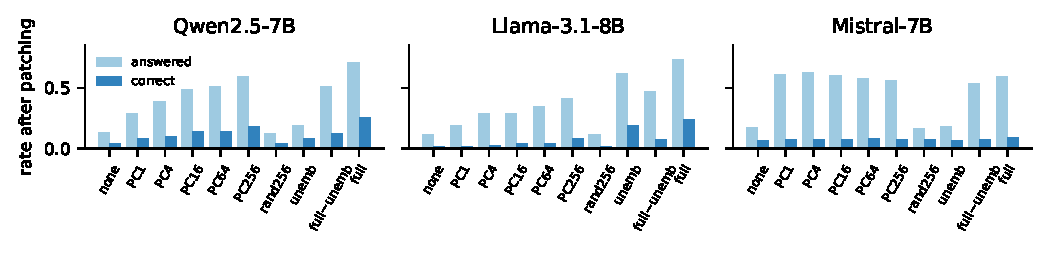
\includegraphics[width=0.84\linewidth]{subspace_rank}
\caption{The insufficient prompt patched with the sufficient-minus-insufficient update projected on the top-$k$ principal components of training updates, on a random 256-dimensional subspace, on the gold answer's unembedding direction (``unemb''), or on everything but that direction.}
\label{fig:subspace}
\end{figure*}

The answering rate rises gradually with $k$ (Qwen: $0.29$ at $k{=}1$, $0.49$ at $k{=}16$, $0.59$ at $k{=}256$, $0.71$ for the full update), while the random 256-dimensional subspace does nothing. Correctness needs even more of the update than answering does. The first component carries much of the switch between answering and abstaining, which is consistent with the projection-out result for $\vdm$. What carries correctness differs by model. On Llama the gold answer's unembedding direction alone restores $0.19/0.62$ (correct/answered), most of the full effect. On Qwen and Mistral it restores little ($0.09/0.19$, $0.07/0.19$), although removing it from the full patch halves Qwen's correctness ($0.26\to0.13$). Mistral's and the 3--4-hop run's effects are captured by the top principal components instead ($0.56$ and $0.51$ answered at $k{=}256$). The causal content is thus high-dimensional and model-specific, and \cref{app:patch-single} shows that it is concentrated in the later layers.

\section{Single-layer patching}
\label{app:patch-single}
\paragraph{Setup.} As in \cref{sec:causal}, the insufficient prompt's anchor residual is replaced by the sufficient run's (full patch), but at a single layer only instead of every layer from the best one onward.

\paragraph{Results.} Patching only the best sufficiency layer (16 for Qwen) leaves the insufficient prompt unchanged in all variants. Patching only layer 26 with the full sufficient residual restores $0.18/0.62$ (correct/answered), so late-layer anchor content alone suffices to make the model answer.

\section{Adaptive retrieval}
\label{app:adaptive}
The readouts of \cref{sec:readout} are computed before generation, so they can drive retrieval: after each round, read the anchor and decide whether to stop and answer or to retrieve more. We test every learned direction in this role, both as a \emph{stopping rule} and as a \emph{verifier} of the answer given at the stopping round.

\paragraph{Simulation.} Each held-out question is walked along its canonical trajectory, one retrieval round per stage: (1) the matched distractors, (2) the first gold hop, (3) the minimal sufficient context, (4) the sufficient context plus a distractor. A policy that never stops answers from stage 4; an oracle stops at stage 3. At round $k$ a policy reads either the state $h(C_k)$ (state probes) or the update the round produced, $\Delta h=h(C_k)-h(C_{\text{prev}})$ (update probes), projects it on the direction at the direction's best layer, and stops when the projection crosses a threshold. The threshold \emph{and the sign} are chosen on training questions to maximise accuracy at the stopping stage (ties broken by fewer rounds), so each direction is used in whichever reading serves retrieval best. For stability and revision we also report the reading that stops when the probe says the last round \emph{changed the answer}. Baselines: never stop; the oracle; the behavioural rule, which stops at the first round whose greedy answer is not INSUFFICIENT (it needs a generation per round, which the probes do not); and a next-token-entropy threshold calibrated the same way. Accuracy counts abstentions as wrong. Everything is computed from stored activations and behaviour, with no new forward passes. Thresholds are calibrated on the questions the probes were trained on, which makes the probe policies, if anything, slightly over-confident on test questions. The trajectories present gold hops in order, so the simulation measures \emph{when to stop}, not what to retrieve.

\begin{table*}[t]
\centering\scriptsize
\setlength{\tabcolsep}{3pt}
\resizebox{\linewidth}{!}{\begin{tabular}{lcccccc}
\toprule
Stopping rule & \musique{} Qwen & \musique{} Llama & \musique{} Mistral & HotpotQA Qwen & \twowiki{} Qwen & Synthetic Qwen \\
\midrule
\multicolumn{7}{l}{\emph{Baselines}} \\
\quad full context (never stop) & 0.404 (4.00) & 0.385 (4.00) & 0.243 (4.00) & 0.685 (3.99)$^{+}$ & 0.460 (4.00) & 0.966 (3.65)$^{+}$ \\
\quad oracle (stop when sufficient) & 0.475 (3.00) & 0.470 (3.00) & 0.336 (3.00) & 0.740 (3.00)$^{+}$ & 0.583 (3.00) & 0.973 (2.93)$^{+}$ \\
\quad behavioural (first non-INSUFFICIENT) & 0.460 (3.09) & 0.460 (3.09) & 0.318 (3.08) & 0.650 (2.53) & \textbf{0.593 (3.10)} & 0.939 (2.88) \\
\quad next-token entropy & 0.381 (3.85)$^{-}$ & 0.378 (3.96) & 0.261 (3.91) & 0.690 (3.74)$^{+}$ & 0.467 (3.67)$^{-}$ & 0.969 (3.35)$^{+}$ \\
\multicolumn{7}{l}{\emph{State probes, $h(C_k)$}} \\
\quad sufficiency (logistic) & 0.466 (3.13) & 0.448 (3.11) & 0.326 (3.13) & \textbf{0.732 (3.08)$^{+}$} & 0.583 (3.02) & \textbf{0.977 (2.96)$^{+}$} \\
\quad sufficiency ($\vdm$) & 0.407 (3.94) & 0.385 (3.58) & 0.261 (3.63) & 0.690 (3.86)$^{+}$ & 0.463 (3.71) & 0.967 (3.00)$^{+}$ \\
\quad correctness & 0.399 (3.57) & 0.443 (3.51) & 0.284 (3.64) & 0.667 (2.92) & 0.547 (3.42) & 0.964 (3.23)$^{+}$ \\
\quad abstention flag & 0.435 (3.07)$^{-}$ & 0.435 (3.12)$^{-}$ & 0.302 (3.13)$^{-}$ & 0.702 (3.18)$^{-}$$^{+}$ & 0.583 (3.12)$^{-}$ & 0.969 (2.99)$^{-}$$^{+}$ \\
\multicolumn{7}{l}{\emph{Update probes, $\Delta h$ of the round}} \\
\quad sufficiency (logistic) & 0.458 (3.30) & 0.460 (3.09) & 0.316 (3.18) & 0.728 (3.23)$^{+}$ & 0.570 (3.16) & 0.949 (3.32) \\
\quad sufficiency ($\vdm$) & \textbf{0.478 (3.06)$^{+}$} & \textbf{0.468 (2.98)} & \textbf{0.336 (3.00)} & 0.727 (3.07)$^{+}$ & 0.543 (3.32) & 0.970 (3.15)$^{+}$ \\
\quad sufficiency matched & 0.404 (4.00) & 0.385 (4.00)$^{-}$ & 0.243 (4.00) & 0.683 (3.98)$^{+}$ & 0.513 (3.21) & 0.858 (3.22) \\
\quad uptake & 0.417 (3.55) & 0.388 (3.35) & 0.259 (3.47) & 0.683 (3.98) & 0.507 (3.42) & 0.957 (3.07)$^{+}$ \\
\quad correction & 0.404 (3.43) & 0.405 (3.38) & 0.302 (3.53) & 0.667 (2.93) & 0.550 (3.36) & 0.920 (3.19) \\
\quad stability & 0.407 (3.46) & 0.400 (3.42) & 0.243 (4.00)$^{-}$ & 0.685 (3.99)$^{+}$ & 0.543 (3.38) & 0.964 (3.63)$^{+}$ \\
\quad stability, stop when the answer changes & 0.402 (3.99) & 0.385 (4.00) & 0.243 (4.00) & 0.685 (3.99) & 0.457 (3.99) & 0.966 (3.65) \\
\quad revision (stop when the answer changes) & 0.396 (3.13) & 0.363 (3.12) & 0.236 (3.23) & 0.690 (3.90)$^{+}$ & 0.513 (3.07) & 0.934 (3.02) \\
\midrule
test questions & 609 & 600 & 610 & 600 & 300 & 830 \\
\bottomrule
\end{tabular}}
\caption{Every direction as a stopping rule: accuracy at the stopping round (mean rounds in parentheses), held-out questions of the document split. Bold: best non-oracle rule per column. $^{-}$: the training-optimal reading stops when the projection is \emph{low}. $^{+}$: the 95\% paired bootstrap interval of the accuracy difference to the behavioural rule lies above zero (1{,}000 resamples of test questions).}
\label{tab:adaptive}
\end{table*}

\paragraph{Stopping rules (\cref{tab:adaptive}, \cref{fig:adaptive}).} Only the sufficiency signals are useful stopping rules. The update-sufficiency $\vdm$ direction is the best learned rule on all three \musique{} models ($0.478$, $0.468$, $0.336$). It matches the oracle ($0.475$, $0.470$, $0.336$) in about three rounds, and on Qwen it is the one rule significantly better than the behavioural rule. The logistic state and update sufficiency probes are statistically tied with the behavioural rule on \musique{}, while acting before any generation. On HotpotQA both beat it ($0.732$ and $0.728$ vs $0.650$), and on the synthetic data the state probe does ($0.977$ vs $0.939$), because the behavioural rule stops too early there (HotpotQA: $2.53$ rounds). On \twowiki{} they tie it ($0.583$ vs $0.593$). The other directions are weak stopping rules on every source. Uptake, correction and stability are trained on decisive or already-correct increments and say nothing about whether the evidence is complete. Their best thresholds stay within $0.06$ of the never-stop policy on \musique{} ($0.24$--$0.42$) and below the best sufficiency rule on every source. Read as ``stop when the answer changes'', stability never fires (about $4.0$ rounds, at full-context accuracy). Revision, the direct change detector, stops at about three rounds but often on the first wrong answer, and is the worst learned rule on \musique{} ($0.236$--$0.396$). The $\vdm$ direction of the \emph{state}, which the causal analysis identified as an abstention gate (\cref{sec:causal}), is a poor stopping rule ($0.26$--$0.41$ on \musique{}). Its update counterpart is the best one. \Cref{fig:adaptive} sweeps each threshold on test questions: the sufficiency curves peak at the oracle's operating point, while the uptake and stability curves rise roughly monotonically towards the full-context accuracy and never cross the behavioural rule on \musique{}.

\begin{figure*}[t]
\centering
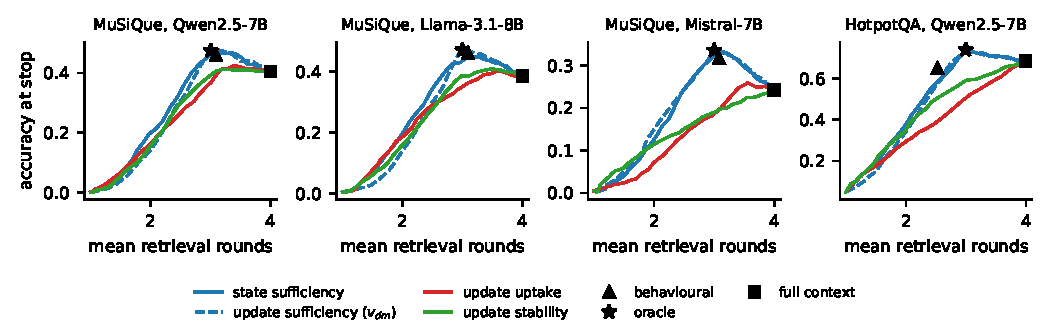
\includegraphics[width=\linewidth]{adaptive_curves}
\caption{Accuracy against mean retrieval rounds when each direction's stopping threshold is swept over test questions (41 quantiles), with the behavioural rule, oracle and full context as points.}
\label{fig:adaptive}
\end{figure*}

\paragraph{Verification at the stopping round (\cref{tab:adaptive_verify}).} The directions that fail as stopping rules are useful once retrieval has stopped. We take the stopping round chosen by the state-sufficiency rule and ask, among the questions the model answers there, how well each signal ranks correct above wrong answers. This is the decision to output, flag or re-retrieve. The uptake direction is the best learned verifier on \musique{} Qwen ($0.672$) and \twowiki{} ($0.847$), where it beats output confidence (top-token probability $0.621$, $0.705$). Correction is the best learned verifier on Mistral ($0.666$ vs $0.630$). By AUROC, next-token entropy is ahead on Llama and HotpotQA (by $0.02$) and on the synthetic data (by $0.11$, where $99\%$ of answered stops are correct). For selective answering, keeping only the more confident half of the answers, uptake gives higher accuracy than top-token probability in five of six settings ($0.789$ vs $0.751$ on \musique{} Qwen, $0.957$ vs $0.870$ on \twowiki{}), and is level on the synthetic data ($0.995$ vs $0.998$). The sufficiency directions are near chance as verifiers on \musique{} and HotpotQA ($0.46$--$0.60$), and the abstention flag is below chance everywhere. They detect completeness, which the stopping rule has already selected for, not whether the answer is right. This division of labour mirrors the readout results. Sufficiency tells the system when the evidence is complete. Uptake, nearly orthogonal to it (\cref{sec:readout}), tells whether the model has actually integrated that evidence into its answer.

\begin{table*}[t]
\centering\scriptsize
\setlength{\tabcolsep}{3pt}
\resizebox{\linewidth}{!}{\begin{tabular}{lcccccc}
\toprule
Signal at the stopping round & \musique{} Qwen & \musique{} Llama & \musique{} Mistral & HotpotQA Qwen & \twowiki{} Qwen & Synthetic Qwen \\
\midrule
top-token probability & 0.621 & 0.615 & 0.630 & 0.654 & 0.705 & 0.876 \\
$-$next-token entropy & 0.623 & \textbf{0.630} & 0.637 & \textbf{0.657} & 0.705 & \textbf{0.877} \\
state: sufficiency & 0.465 & 0.463 & 0.521 & 0.526 & 0.621 & 0.738 \\
state: correctness & 0.560 & 0.568 & 0.618 & 0.626 & 0.763 & 0.388 \\
state: abstention flag & 0.432 & 0.473 & 0.412 & 0.395 & 0.444 & 0.252 \\
update: sufficiency & 0.482 & 0.543 & 0.495 & 0.554 & 0.594 & 0.585 \\
update: sufficiency ($\vdm$) & 0.566 & 0.569 & 0.601 & 0.567 & 0.806 & 0.534 \\
update: uptake & \textbf{0.672} & 0.613 & 0.647 & 0.617 & \textbf{0.847} & 0.764 \\
update: correction & 0.594 & 0.576 & \textbf{0.666} & 0.639 & 0.753 & 0.400 \\
update: stability & 0.549 & 0.566 & 0.559 & 0.562 & 0.775 & 0.497 \\
update: revision & 0.512 & 0.517 & 0.490 & 0.524 & 0.601 & 0.531 \\
\midrule
accuracy of all answered stops & 0.665 & 0.666 & 0.534 & 0.810 & 0.761 & 0.990 \\
accuracy, top half by top-token prob. & 0.751 & 0.733 & 0.618 & 0.863 & 0.870 & 0.998 \\
accuracy, top half by uptake & 0.789 & 0.757 & 0.651 & 0.867 & 0.957 & 0.995 \\
answered stops & 427 & 404 & 373 & 542 & 230 & 819 \\
\bottomrule
\end{tabular}}
\caption{Verification once retrieval stops (state-sufficiency stopping rule): AUROC of each signal at the stopping round for the correctness of the answer given there (answered stops only). Bold: best per column. Bottom: accuracy of all answered stops and of the half ranked highest by top-token probability or by the uptake direction.}
\label{tab:adaptive_verify}
\end{table*}

\paragraph{Other sources.} On 3--4-hop \musique{} the trajectories end at the sufficient context (no post-sufficiency stage), so the oracle and the never-stop policy coincide ($0.360$). All learned rules reach this value, while the behavioural rule stops too early ($0.340$). On RAGBench (relation split, 955 test questions) most trajectories have two or three stages and no distractor after sufficiency, and every policy lies within $0.21$--$0.23$. With the original protocol of a threshold at $0.97$ training precision, the state-sufficiency rule reached $0.442$ in $2.87$ rounds on \musique{} Qwen and $0.707$ in $2.90$ on HotpotQA. Accuracy-optimal calibration trades a few rounds for accuracy on \musique{}.

\section{Results by question group on the external sources}
\label{app:groups}
\Cref{tab:groups} breaks down the held-out probe AUROC of the external sources (\cref{sec:external}) by question group, to separate the evidence-state readout from properties of the questions. The groups are: closed-book status (unlike the main runs, HotpotQA and RAGBench keep the questions the model answers correctly without evidence); question type (HotpotQA bridge versus comparison, whose two facts are independent lookups); domain (RAGBench's twelve sub-datasets grouped into biomedical, finance, technical, customer support, general web QA and Wikipedia); and hop count (synthetic 1--3 hops; for RAGBench, one versus two gold documents). The stored best-layer probe of each source, trained on all groups, is scored per group on test questions without refitting; increment counts are in parentheses.
\begin{table*}[t]
\centering\scriptsize
\begin{tabular}{lllccc}
\toprule
Dataset & grouping & group & sufficiency & uptake & correction \\
\midrule
HotpotQA & closed book & incorrect & 0.978 (7840) & 0.724 (986) & 0.839 (5554) \\
HotpotQA & closed book & correct & 0.984 (1689) & 0.802 (214) & 0.885 (760) \\
HotpotQA & qtype & bridge & 0.978 (7878) & 0.680 (982) & 0.839 (4963) \\
HotpotQA & qtype & comparison & 0.985 (1651) & 0.787 (218) & 0.880 (1351) \\
RAGBench & domain & biomedical & 0.929 (1473) & 0.776 (291) & 0.818 (1331) \\
RAGBench & domain & finance & 0.899 (1081) & 0.641 (206) & 0.769 (949) \\
RAGBench & domain & technical & 0.881 (1069) & 0.675 (196) & 0.733 (989) \\
RAGBench & domain & customer support & 0.897 (716) & 0.569 (153) & 0.658 (587) \\
RAGBench & domain & general & 0.835 (1821) & 0.721 (352) & 0.702 (1520) \\
RAGBench & domain & wikipedia & 0.978 (729) & 0.557 (158) & 0.766 (612) \\
RAGBench & n hops & 1 & 0.836 (2476) & 0.698 (444) & 0.785 (2211) \\
RAGBench & n hops & 2 & 0.931 (4413) & 0.677 (912) & 0.711 (3777) \\
Synthetic & n hops & 1 & 0.922 (3645) & 0.992 (486) & 0.875 (2450) \\
Synthetic & n hops & 2 & 0.970 (6192) & 0.928 (1032) & 0.926 (4929) \\
Synthetic & n hops & 3 & 0.970 (11501) & 0.916 (2395) & 0.931 (8859) \\
\bottomrule
\end{tabular}
\caption{Held-out probe AUROC by question group (test-set increment counts in parentheses): closed-book status, question type, domain and hop count.}
\label{tab:groups}
\end{table*}

\section{The Evidence State Transition Benchmark}
\label{app:estb}

The Evidence State Transition Benchmark (ESTB) tests whether the evidence-state readout and its causal profile, established on \musique{} trajectories in \cref{sec:readout,sec:causal}, survive controlled changes to the evidence. It puts all of our sources under one labelling scheme and one evaluation protocol. This appendix describes what the benchmark measures, how each axis was built, and the full results of the retrieval-source and linguistic-form runs, which appear only in summary in \cref{sec:external}.

\subsection{What the benchmark measures}
\label{app:estb-measures}

\paragraph{Unit of measurement.} As in the rest of the paper, the unit is an \emph{evidence state transition}: an increment $C_{k-1}\to C_k$ that adds one paragraph (or, for post-sufficiency and full-context increments, a set of paragraphs) to the context, with the paired update $\Delta h=h(C_k)-h(C_{k-1})$ read at the answer-start anchor. ESTB annotates every increment with the \emph{quality state} of the evidence it adds (\cref{tab:estb-states}) and with the values of the other axes (\cref{tab:estb-axes}): retrieval source, linguistic form, domain, question type, hop count and closed-book status.

\paragraph{Labels.} Each increment carries the sufficiency label $y^{\mathrm{suff}}=\mathbf 1[C_k\text{ sufficient},\,C_{k-1}\text{ not}]$, which is defined by construction from the gold hops and does not depend on the model, and a behavioural uptake label for increments that cross sufficiency (answer becomes correct or not). An increment crosses sufficiency exactly when it supplies the last missing hop, whether in the original wording (C3), paraphrased, or from an independently authored source.

\paragraph{Measurements per cell.} A \emph{cell} is the set of increments of one run that share one value on one axis (for example, ``E5-retrieved distractors, quality state C1''). For every cell we report:
\begin{enumerate}
  \item \textbf{Within-run readout:} the test AUROC of the run's own held-out probe (trained on the run's training questions), for sufficiency, matched sufficiency and uptake. This is the ceiling: is the state linearly decodable at all under this kind of evidence?
  \item \textbf{Transfer without retraining:} the AUROC of the Qwen \musique{} two-hop direction (document split, at its best layer), applied unchanged. Because the ESTB runs sample from the same \musique{} pool as the source run, 818 of the 1{,}200 questions in the benchmark-gold runs (273 of 402 and 152 of 219 in the fully retrieved runs) are in the source probe's training split. These questions are \emph{excluded} from every transfer score, so transfer is measured only on questions the source probe never saw.
  \item \textbf{Quality-state separability:} for each quality state $Q$, the AUROC separating $Q$'s increments (negatives) from the decisive increments of the same run (positives). Near $1$, the readout cleanly distinguishes $Q$ from completing the evidence; lower values mean that $Q$ looks like sufficiency to the probe.
  \item \textbf{Causal profile:} on 150 held-out questions, the answered rate of the insufficient prompt unpatched, with the full sufficient anchor residual patched in, and with only the probe-direction component ($\parallel v$) patched in, all at every layer from the best one onward; and the answered rate of sufficient prompts after projecting $\vdm$ to its insufficient-state value (\cref{sec:causal}).
\end{enumerate}
The benchmark therefore separates three questions: whether the state is \emph{present} (1), whether it is the \emph{same} state as on \musique{} (2, 3), and whether its causal profile, an inert probe direction alongside a causally sufficient anchor and a $\vdm$ abstention gate, carries over (4).

\paragraph{What the benchmark does not measure.} ESTB does not score answer quality or retrieval quality for their own sake: retrieval and paraphrasing only vary the evidence that enters a trajectory. It does not ask whether the model \emph{should} answer from partial or contradictory evidence; those states are scored by whether the readout separates them from genuine completion. The sufficiency label is structural (all hops present) rather than semantic, so a passage that happens to state a fact in a way our string-based labelling misses (\cref{app:estb-limits}) is counted as insufficient.

\subsection{Evidence quality states}
\label{app:estb-quality}

\Cref{tab:estb-states} lists the seven quality states of the evidence-quality axis and the increment kinds (\cref{app:conditions}) that realise them. All states except C0 are increments, i.e.\ transitions \emph{into} the state from the preceding context.

\begin{table*}[t]
\centering\scriptsize
\setlength{\tabcolsep}{3pt}
\begin{tabular}{llp{6.4cm}c}
\toprule
State & Name & Increment kinds (added evidence) & $y^{\mathrm{suff}}$ \\
\midrule
C0 & none & no evidence (start state of every trajectory) & -- \\
C1 & irrelevant & \texttt{distractor\_from\_none}, \texttt{distractor}: a length-matched distractor added to an empty or penultimate context & 0 \\
C2 & partial & \texttt{gold\_nondecisive}: a gold hop that leaves another hop missing; \texttt{partial}: the decisive paragraph rewritten to withhold its value; \texttt{redundant} from a penultimate state (C2+redundant) & 0 \\
C3 & complete & \texttt{decisive}, \texttt{loo\_decisive}: the last missing hop; \texttt{decisive\_paraphrase}, \texttt{decisive\_independent}: the same hop paraphrased or from an independent source & 1 \\
C4 & complete + redundant & \texttt{post\_distractor}, \texttt{post\_redundant}, \texttt{post\_redundant\_paraphrase}, \texttt{post\_redundant\_independent}, \texttt{full\_context}: further evidence added after sufficiency & 0 \\
C5 & contradictory & \texttt{false}: the decisive hop with its value replaced (from a penultimate state); \texttt{post\_false}: a falsified copy added to a sufficient context & 0 \\
C6 & answer string, no relation & \texttt{answer\_ctrl}: a distractor with ``(Not to be confused with \{answer\}.)'' appended & 0 \\
\bottomrule
\end{tabular}
\caption{ESTB evidence-quality states and the increment kinds that realise them. $y^{\mathrm{suff}}$: whether the increment crosses into sufficiency.}
\label{tab:estb-states}
\end{table*}

The contradictory state has two sources. On benchmark and retrieved trajectories, the false value is another question's sub-answer of the same relation type (\texttt{false\_synthetic}); on the synthetic benchmark, it is a generated value of the same type. The tables label the first kind ``C5 contradictory (synthetic)'' because the false value is substituted rather than found in a real document; naturally occurring contradictions are not separated from \texttt{near\_miss} passages by our labelling (\cref{app:estb-limits}). Partial evidence is defined in two ways: for multi-hop questions, a gold hop that leaves another hop missing (``partial (hop)''); for any question, the decisive paragraph rewritten so that its subject and relation remain but the value is withheld (``partial (masked)'', \cref{app:estb-form}).

\subsection{Axes and sources}
\label{app:estb-axes}

\begin{table*}[t]
\centering\scriptsize
\setlength{\tabcolsep}{3pt}
\begin{tabular}{lp{4.1cm}p{6.1cm}}
\toprule
Axis & Levels & Source (runs) \\
\midrule
Evidence quality & C0--C6 (\cref{tab:estb-states}) & every run \\
Retrieval source & benchmark; BM25; E5 (dense); each as distractors only or as all evidence & \musique{} 2-hop rebuilt over wiki-18 (\cref{app:estb-retrieval}) \\
Linguistic form & verbatim; LLM paraphrase; independently authored; templated (5 families) & \musique{} variants run (\cref{app:estb-form}); synthetic benchmark \\
Domain & Wikipedia; biomedical; finance; technical; customer support; general web QA & \musique{}, HotpotQA, \twowiki{}; RAGBench's 12 sub-datasets \\
Question type & bridge; comparison; single-hop & HotpotQA; RAGBench; synthetic \\
Hop count & 1; 2; 3--4 & synthetic, RAGBench; \musique{} 2-hop; \musique{} 3--4-hop \\
Closed-book status & correct; incorrect & HotpotQA and RAGBench (\texttt{select: all}) \\
\bottomrule
\end{tabular}
\caption{ESTB axes. The domain, question-type, hop-count and closed-book axes reuse the external runs of \cref{sec:external}, scored per group in \cref{app:groups}; the retrieval-source and linguistic-form axes required new construction and are detailed here.}
\label{tab:estb-axes}
\end{table*}

All ESTB runs reported here use Qwen2.5-7B-Instruct \cite{qwen2025qwen25} and the pipeline of the main text without modification. The four retrieval runs and the variants run draw 1{,}200 two-hop \musique{} training questions that the model answers incorrectly closed-book, with no random hop permutations.

\subsection{Retrieval-source axis}
\label{app:estb-retrieval}

\paragraph{Corpus and retrievers.} Evidence comes from wiki-18, the December 2018 Wikipedia dump of \citet{karpukhin2020dense} as distributed with FlashRAG \cite{jin2025flashrag}: 21M passages of 100 words with their article titles. \emph{BM25} \cite{robertson2009bm25}, a lexical retriever, uses the \texttt{bm25s} implementation \cite{lu2024bm25s} over title and text, with English stop-words and Snowball stemming. \emph{E5} \cite{wang2022e5}, a dense retriever, uses the published FAISS flat inner-product index of \texttt{e5-base-v2} passage embeddings; queries are encoded with the \texttt{query:} prefix and mean pooling, then $\ell_2$-normalised.

\paragraph{Queries.} A single question-level query rarely retrieves both hops of a bridge question. Each question therefore issues the question itself plus one query per hop, taken from \musique{}'s decomposition with the earlier hops' sub-answers substituted for the \texttt{\#k} placeholders (three queries per two-hop question). This imitates an iterative or decomposing RAG system that gets the earlier hops right. The per-query hit lists are merged round-robin by rank, de-duplicated, and cut at $k=30$ passages per question.

\paragraph{Passage labels.} Each retrieved passage is labelled against the question's gold hops by title and string matching (titles normalised by lower-casing and removing a trailing parenthetical):
\begin{itemize}
  \item \texttt{retrieved\_gold}: the title matches a gold hop's page \emph{and} the passage contains that hop's sub-answer;
  \item \texttt{same\_page}: the title matches a gold hop's page but the sub-answer is absent, i.e.\ partial evidence found in the wild;
  \item \texttt{near\_miss}: not a gold page, but the passage mentions a bridge entity or the final answer, which is the natural analogue of the answer-string control C6;
  \item \texttt{irrelevant}: everything else.
\end{itemize}
\Cref{tab:estb-retrieval} gives the label composition. E5 retrieves at least one gold passage for $85.5\%$ of questions and both hops for $33.5\%$; BM25 does so for $68.1\%$ and $18.2\%$.

\begin{table*}[t]
\centering\small
\begin{tabular}{lcccccc}
\toprule
& \multicolumn{4}{c}{retrieved passages (top 30)} & \multicolumn{2}{c}{questions with gold for} \\
\cmidrule(lr){2-5}\cmidrule(lr){6-7}
Retriever & gold & same page & near miss & irrelevant & $\ge1$ hop & both hops \\
\midrule
E5 & 0.080 & 0.139 & 0.292 & 0.489 & 0.855 & 0.335 \\
BM25 & 0.053 & 0.080 & 0.331 & 0.535 & 0.681 & 0.182 \\
\midrule
\multicolumn{7}{l}{Distractors used in the trajectories (18 per question): same page / near miss / irrelevant} \\
E5 & \multicolumn{6}{l}{0.231 / 0.460 / 0.309} \\
BM25 & \multicolumn{6}{l}{0.133 / 0.535 / 0.332} \\
\bottomrule
\end{tabular}
\caption{Retrieved passages by label (1{,}200 \musique{} two-hop questions, multi-query retrieval, $k=30$).}
\label{tab:estb-retrieval}
\end{table*}

\paragraph{Trajectories.} Two modes turn retrieval output into trajectories.
\begin{itemize}
  \item \textbf{Retrieved distractors} (\emph{noise} mode): the benchmark gold paragraphs are kept and every distractor is replaced by a retrieved non-gold passage. The 18 distractors per question are taken hardest first: same-page passages, then near misses, then irrelevant passages, each in rank order. The trajectory builder then draws length-matched distractors from this pool exactly as it does from the benchmark pool. Distractors are thus no longer the benchmark's curated negatives but what a retriever returns for the same question, and nearly a quarter of E5's distractors come from the gold pages themselves.
  \item \textbf{All evidence retrieved} (\emph{full} mode): the gold paragraph of each hop is also replaced, by the highest-ranked \texttt{retrieved\_gold} passage for that hop, so every paragraph the model sees is a 100-word wiki-18 passage. Only questions with a retrieved gold passage for both hops can be used: 402 for E5 and 219 for BM25.
\end{itemize}
Every other part of the construction (chains, controls, falsification, answer-string hatnotes, post-sufficiency and full-context increments) is unchanged, which yields the full set of quality states over retrieved evidence: 20{,}400 increments in each noise run, 6{,}809 (E5) and 3{,}703 (BM25) in the full runs.

\subsection{Linguistic-form axis}
\label{app:estb-form}

\paragraph{LLM paraphrase and partial variants.} For every gold hop paragraph of the 1{,}200 questions, Qwen2.5-7B-Instruct generates two rewrites by greedy decoding (at most 220 tokens):
\begin{itemize}
  \item \emph{paraphrase}: ``Rewrite the following encyclopedia paragraph in completely different wording and sentence structure, keeping every fact exactly the same. You must keep the exact string `\{sub-answer\}' verbatim.''
  \item \emph{partial}: ``Rewrite the following encyclopedia paragraph so that it still talks about `\{subject\}' and the same topic, but withholds the specific fact `\{sub-answer\}': do not mention `\{sub-answer\}' or any equivalent name or value anywhere; instead say that the detail is not recorded here.''
\end{itemize}
Generations are validated before use. A paraphrase is kept only if it contains the sub-answer, is between $0.5\times$ and $2\times$ the original's length, and shares fewer than $60\%$ of its word 4-grams with the original. A partial is kept only if it contains neither the sub-answer, nor the final answer, nor any answer alias, has at least 15 words, and still mentions the hop's subject. Of 2{,}400 hop paragraphs, 2{,}180 ($90.8\%$) yield a valid paraphrase and 1{,}411 ($58.8\%$) a valid partial.

\paragraph{Independently authored sources.} \musique{}, HotpotQA and \twowiki{} all take paragraphs from Wikipedia, but from different dumps, with different paragraph boundaries and often different revisions. For each \musique{} gold hop with page title $T$ and sub-answer $a$, we search the gold and distractor paragraphs of the \emph{other} two datasets for one whose normalised title is $T$, that contains $a$, and that shares fewer than $60\%$ of its 4-grams with the \musique{} paragraph; when several qualify, the least overlapping is used. This finds an independently written statement of the same relation for 228 of the 2{,}400 hops (144 from HotpotQA, 84 from \twowiki{}).

\paragraph{Increments.} From the penultimate state, the paraphrased and independent paragraphs give \texttt{decisive\_paraphrase} and \texttt{decisive\_independent} increments (C3, crossing sufficiency), and the partial paragraph gives a \texttt{partial} increment (C2, which does not). After sufficiency, the paraphrase or independent version of a hop already present gives \texttt{post\_redundant\_paraphrase} and \texttt{post\_redundant\_independent} increments (C4). Together with the standard kinds, the variants run has 25{,}632 increments, including 2{,}180 paraphrased decisive, 228 independent decisive and 1{,}411 partial ones.

\paragraph{Synthetic templated form.} The synthetic benchmark (\cref{sec:external}) supplies the fully controlled end of the axis: fictional entities over seven relations (founder, birthplace, capital, spouse, award, employer, headquarters), five template families per relation, one to three hops, and for every gold fact a paraphrase, a partial (value withheld) and a contradictory (different value) variant, with near-miss distractors (same relation, other subject; same subject, other relation) and unrelated filler.

\subsection{Results}
\label{app:estb-results}

\begin{table*}[t]
\centering\scriptsize
\setlength{\tabcolsep}{2.5pt}
\resizebox{\linewidth}{!}{\begin{tabular}{lrccccccccc}
\toprule
& & \multicolumn{3}{c}{within-run probe (AUROC)} & \multicolumn{2}{c}{MuSiQue dir.} & \multicolumn{4}{c}{answered rate} \\
\cmidrule(lr){3-5}\cmidrule(lr){6-7}\cmidrule(lr){8-11}
Evidence source & $n_q$ & suff. & matched & uptake & suff. & uptake & unpatched & full & $\parallel v$ & proj.-out $\vdm$ \\
\midrule
Benchmark gold + benchmark distractors & 2000 & 0.948 & 0.911 & 0.775 & (source) & (source) & 0.13 & 0.71 & 0.13 & 0.01 \\
Gold + E5-retrieved distractors & 1200 & 0.946 & 0.909 & 0.681 & 0.935 & 0.817 & 0.10 & 0.77 & 0.10 & 0.02 \\
Gold + BM25-retrieved distractors & 1200 & 0.951 & 0.915 & 0.679 & 0.939 & 0.817 & 0.10 & 0.77 & 0.10 & 0.01 \\
All evidence E5-retrieved & 402 & 0.922 & 0.891 & 0.839 & 0.905 & 0.762 & 0.19 & 0.72 & 0.19 & 0.03 \\
All evidence BM25-retrieved & 219 & 0.912 & 0.876 & 0.748 & 0.910 & 0.820 & 0.30 & 0.68 & 0.30 & 0.02 \\
+ LLM paraphrase / partial / independent & 1200 & 0.935 & 0.885 & 0.718 & 0.929 & 0.796 & 0.10 & 0.77 & 0.10 & 0.00 \\
\bottomrule
\end{tabular}}
\caption{Retrieval-source and linguistic-form axes (Qwen2.5-7B, \musique{} 2-hop). Within-run probes on the document split, except the two fully retrieved runs (question split, too few questions for document components). \musique{} direction: transfer without retraining, scored only on questions outside the source probe's training split. Answered rate: the insufficient prompt unpatched, with the full sufficient anchor, and with only the probe-direction component; and the sufficient prompt with $\vdm$ projected to its insufficient value.}
\label{tab:estb}
\end{table*}

\paragraph{Retrieval source.} With retrieved distractors (\cref{tab:estb}), within-run sufficiency is unchanged ($0.946$ E5, $0.951$ BM25, against $0.948$ with benchmark distractors), and the \musique{} direction transfers at $0.935$/$0.939$ on source-unseen questions. Retrieved distractors are harder than the benchmark's: the transferred direction separates C1 increments from decisive ones at $0.906$ (E5) and $0.917$ (BM25), against $0.945$ for benchmark distractors, and answer-string controls at $0.962$/$0.971$ against $0.982$. The run's own probe recovers most of this ($0.972$/$0.982$ for C1), so the drop is a shift in the distractor distribution rather than a loss of the state. Uptake falls within run ($0.68$, against $0.78$), but the transferred \musique{} uptake direction scores $0.817$ on the same increments: these runs have 1{,}200 rather than 2{,}000 questions, so the within-run probe is trained on fewer decisive increments, which is the likely reason. With all evidence retrieved, sufficiency stays at $0.91$--$0.92$ within run and $0.905$--$0.910$ transferred, and C1 separability is the lowest of any run ($0.84$ transferred, $0.89$--$0.92$ own), which is expected when every paragraph is a 100-word passage from the same corpus as the gold ones. In every retrieval cell the causal profile of \cref{sec:causal} reproduces: the full anchor patch raises answering from $0.10$--$0.30$ to $0.68$--$0.77$, the probe-direction component leaves it exactly at the unpatched rate, and projecting out $\vdm$ leaves $0.01$--$0.03$ answered.

\begin{table*}[t]
\centering\small
\begin{tabular}{lrcc}
\toprule
Quality state vs.\ decisive increment & $n$ & own probe & MuSiQue dir. \\
\midrule
C5 contradictory (synthetic) & 764 & 0.762 & 0.725 \\
C2 partial (masked) & 436 & 0.809 & 0.736 \\
C1 irrelevant & 1146 & 0.942 & 0.941 \\
C4 complete+paraphrase & 381 & 0.974 & 0.952 \\
C6 answer string, no relation & 764 & 0.975 & 0.979 \\
C2+redundant & 764 & 0.982 & 0.978 \\
C4 complete+independent & 57 & 0.995 & 0.950 \\
C4 complete+irrelevant & 382 & 0.997 & 0.980 \\
C4 complete+redundant & 382 & 0.999 & 0.984 \\
C5 complete+contradictory & 382 & 1.000 & 0.994 \\
C2 partial (hop) & 764 & 1.000 & 0.996 \\
C4 full context & 382 & 1.000 & 0.999 \\
\bottomrule
\end{tabular}
\caption{Quality-state separability (\musique{} variants run): AUROC separating each state's increments (negatives) from decisive increments (positives), with the run's own probe (test questions) and with the \musique{} direction (source-unseen questions). Lower values mean the state looks more like completing the evidence.}
\label{tab:estb_quality}
\end{table*}

\paragraph{Linguistic form.} Paraphrased and independently authored decisive paragraphs are read as completing the evidence just as the original wording is. Against all non-decisive increments, the transferred \musique{} direction scores original decisive increments at $0.931$ AUROC, paraphrased ones at $0.929$ and independently authored ones at $0.918$, with mean projections $0.101$, $0.098$ and $0.096$ (non-decisive: $-0.082$). Paraphrastic and independent redundancy after sufficiency is cleanly separated from completion ($0.974$ and $0.995$ own probe, \cref{tab:estb_quality}). The two hardest quality states are the ones that most resemble completion. Contradictory evidence added from the penultimate state (C5, the decisive paragraph with a swapped value) reaches only $0.76$ own and $0.73$ transferred, and it has the same ``supplies the missing relation'' surface form as the decisive paragraph. Masked partial evidence (C2), with subject and relation present but the value withheld, reaches $0.81$ own and $0.74$ transferred; its mean projection ($0.044$) lies between the non-decisive and decisive means. Partial evidence in the multi-hop sense (a non-decisive hop) is separated almost perfectly ($1.00$). Contradictory evidence is the hardest control in every retrieval run as well ($0.71$--$0.75$ transferred) and is also the state that projects closest to completion on the synthetic benchmark (\cref{sec:external}).

\paragraph{Summary.} Across the retrieval-source and linguistic-form axes, the sufficiency state remains decodable ($\ge0.91$), the \musique{} direction transfers to unseen questions ($\ge0.90$), wording and authorship of the decisive evidence do not matter, and the causal dissociation reproduces in every cell. What changes is the difficulty of the controls: retrieved distractors from the gold pages and value-withheld or value-swapped versions of the decisive paragraph are where a deployed sufficiency detector would err.

\subsection{Limitations of the construction}
\label{app:estb-limits}
\begin{itemize}
  \item \textbf{Oracle decomposition.} The per-hop retrieval queries substitute gold sub-answers into \musique{}'s decomposition, so the retriever behaves like an iterative system that solves the earlier hops correctly. Gold coverage is an upper bound on what a realistic multi-hop retriever would achieve.
  \item \textbf{String-based passage labels.} \texttt{retrieved\_gold} requires the gold page title and the sub-answer string. A passage on another page that states the same relation is labelled \texttt{near\_miss} and used as a distractor; a gold-page passage that mentions the sub-answer in an unrelated sentence counts as gold. Both introduce some label noise, in opposite directions.
  \item \textbf{Selection in the fully retrieved runs.} Only questions whose two hops were both retrieved are kept (34\% for E5, 18\% for BM25), which favours questions with lexically salient hops.
  \item \textbf{Self-generated paraphrases.} Paraphrases and partials are generated by the same model that is probed. Validation removes rewrites that drop the sub-answer or copy the original, but generated text may still be easier for the model to read than human-written text. The independently authored paragraphs avoid this but are few (64 decisive increments on source-unseen questions).
  \item \textbf{One model.} All ESTB runs reported here use Qwen2.5-7B-Instruct.
\end{itemize}

\section{Compute and reproducibility}
\label{app:compute}
Collection for one 2-hop model ($\approx35$k conditions) takes about 22 hours on 64 CPU cores (bf16, $\approx300$ prompt tokens/s) or about one hour on an H200 shared with another job; the 3--4-hop run took 1.3 GPU-hours; all causal experiments and text baselines together used about 7 GPU-hours. Probing runs on CPU in one to two hours per model. Every stage is deterministic given the seed (question sampling, insertion positions, false-answer choice, splits) and resumable. Code, configurations and the trajectory construction are released with the paper.


\end{document}
